\section{Mathematical Model}
\label{ch:mathmodel}

As per the base and periodic models shown in \cite{grigor20}.

\subsection{Base model}

\subsubsection{Definitions and Theory}

\subsubsection{How to select the best model}

\subsubsection{Forecasting}

\subsubsection{Implementation in R}

\begin{figure}[H]
\minipage{0.48\textwidth}
  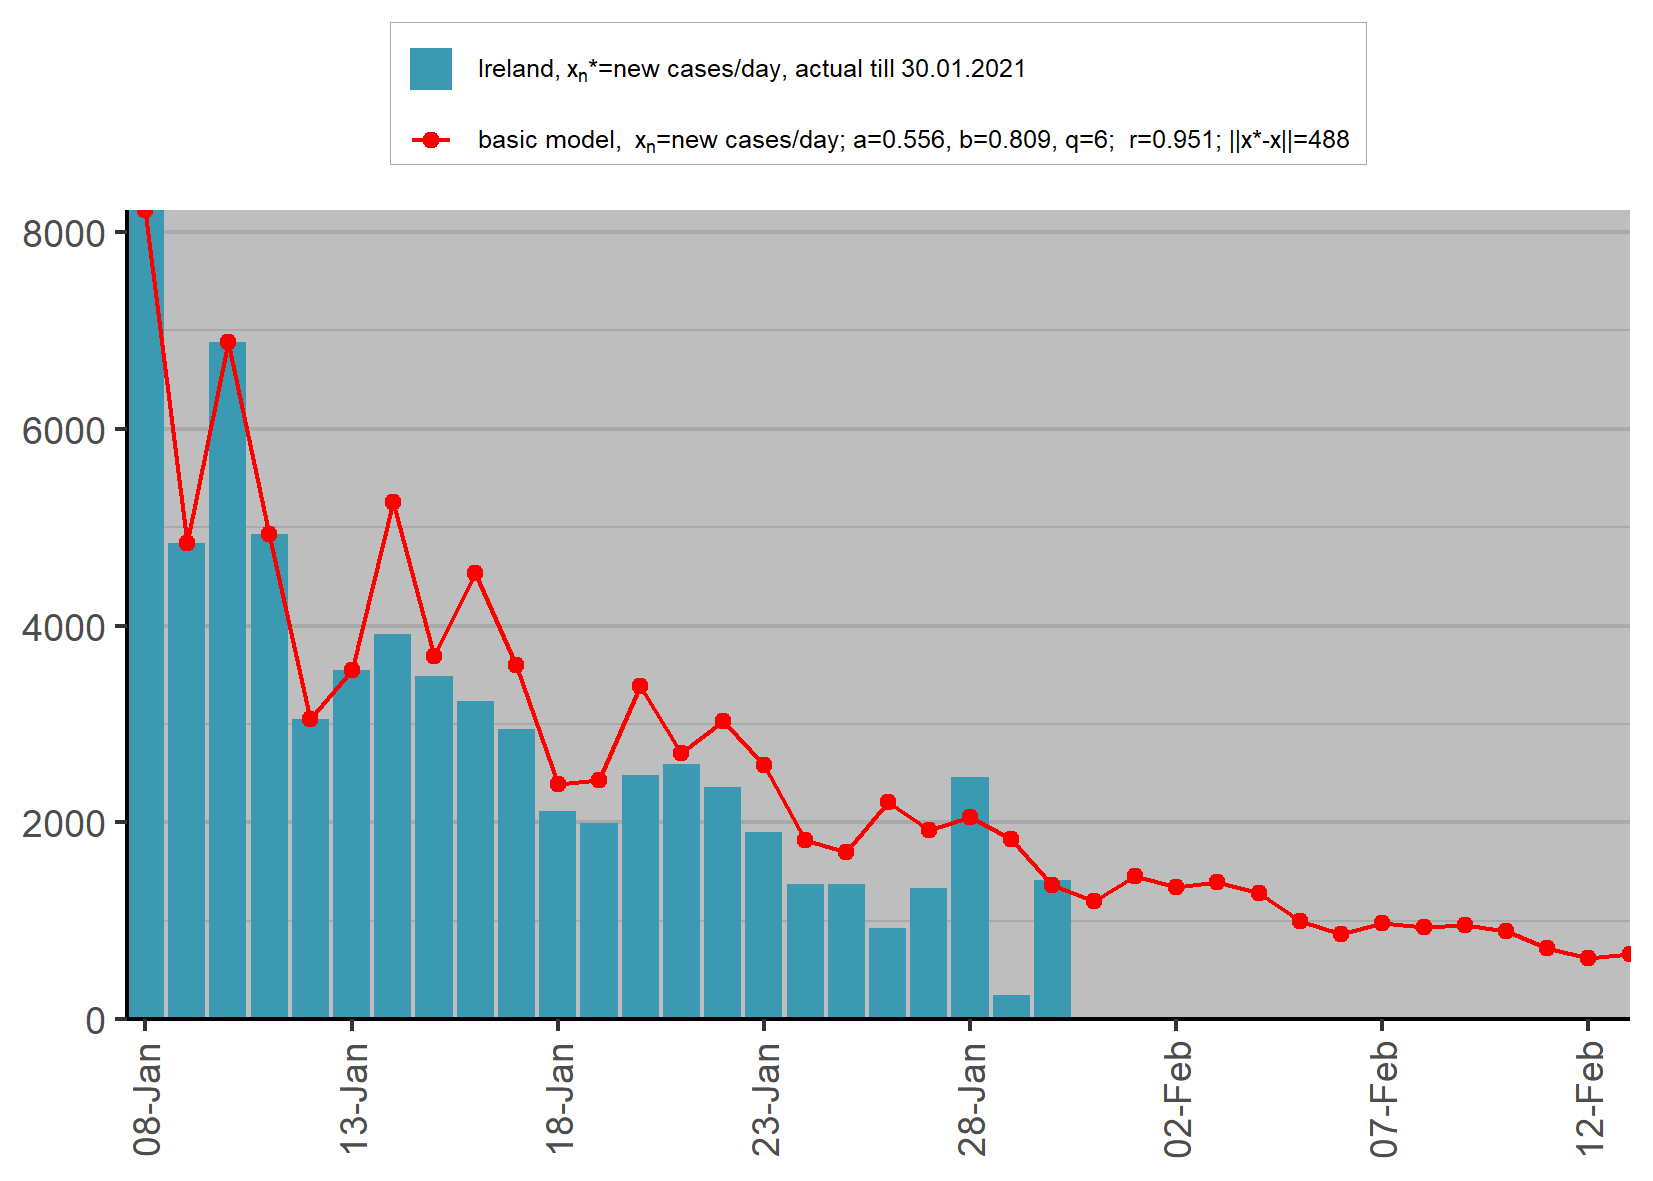
\includegraphics[width=\linewidth]{Ireland-basexn.png} \label{fig:ireland-basexn}
\endminipage\hfill
\minipage{0.48\textwidth}
  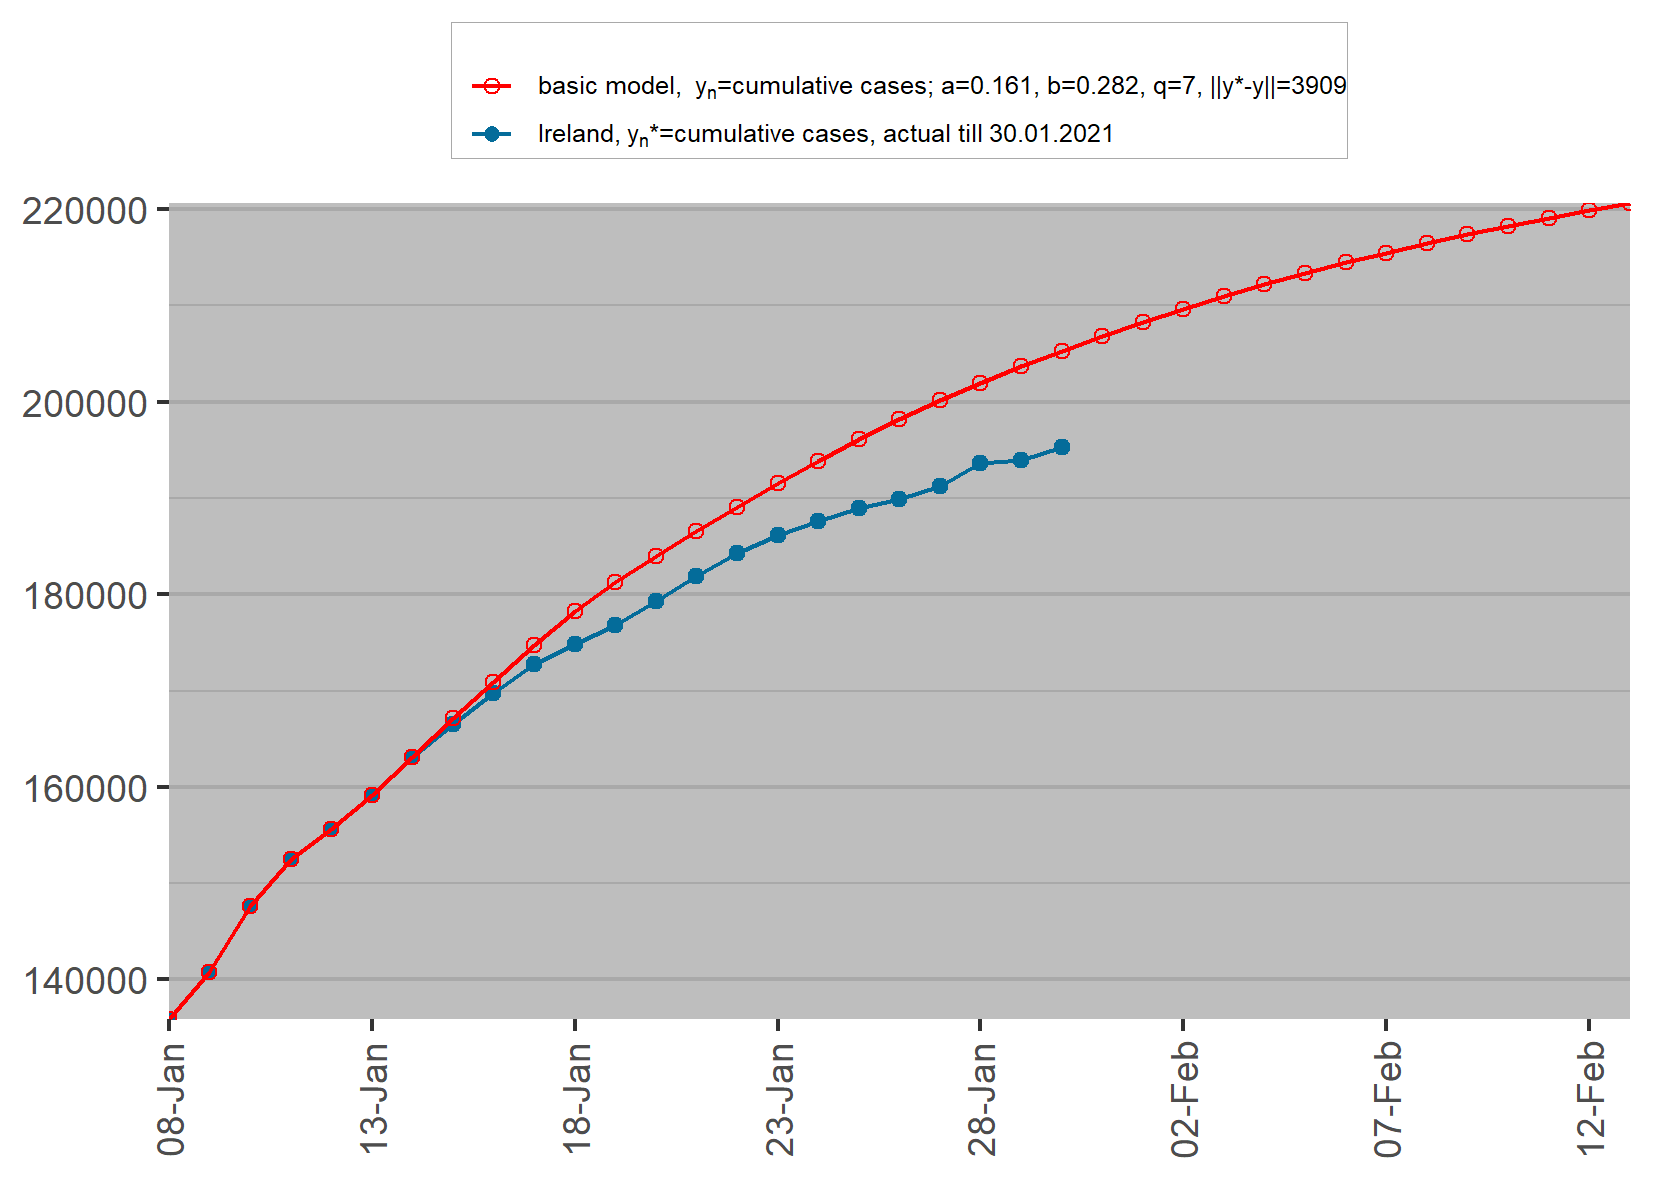
\includegraphics[width=\linewidth]{Ireland-baseyn.png} \label{fig:ireland-baseyn}
\endminipage
\caption{Basic model, Ireland}
\end{figure}

\begin{figure}[H]
\minipage{0.48\textwidth}
  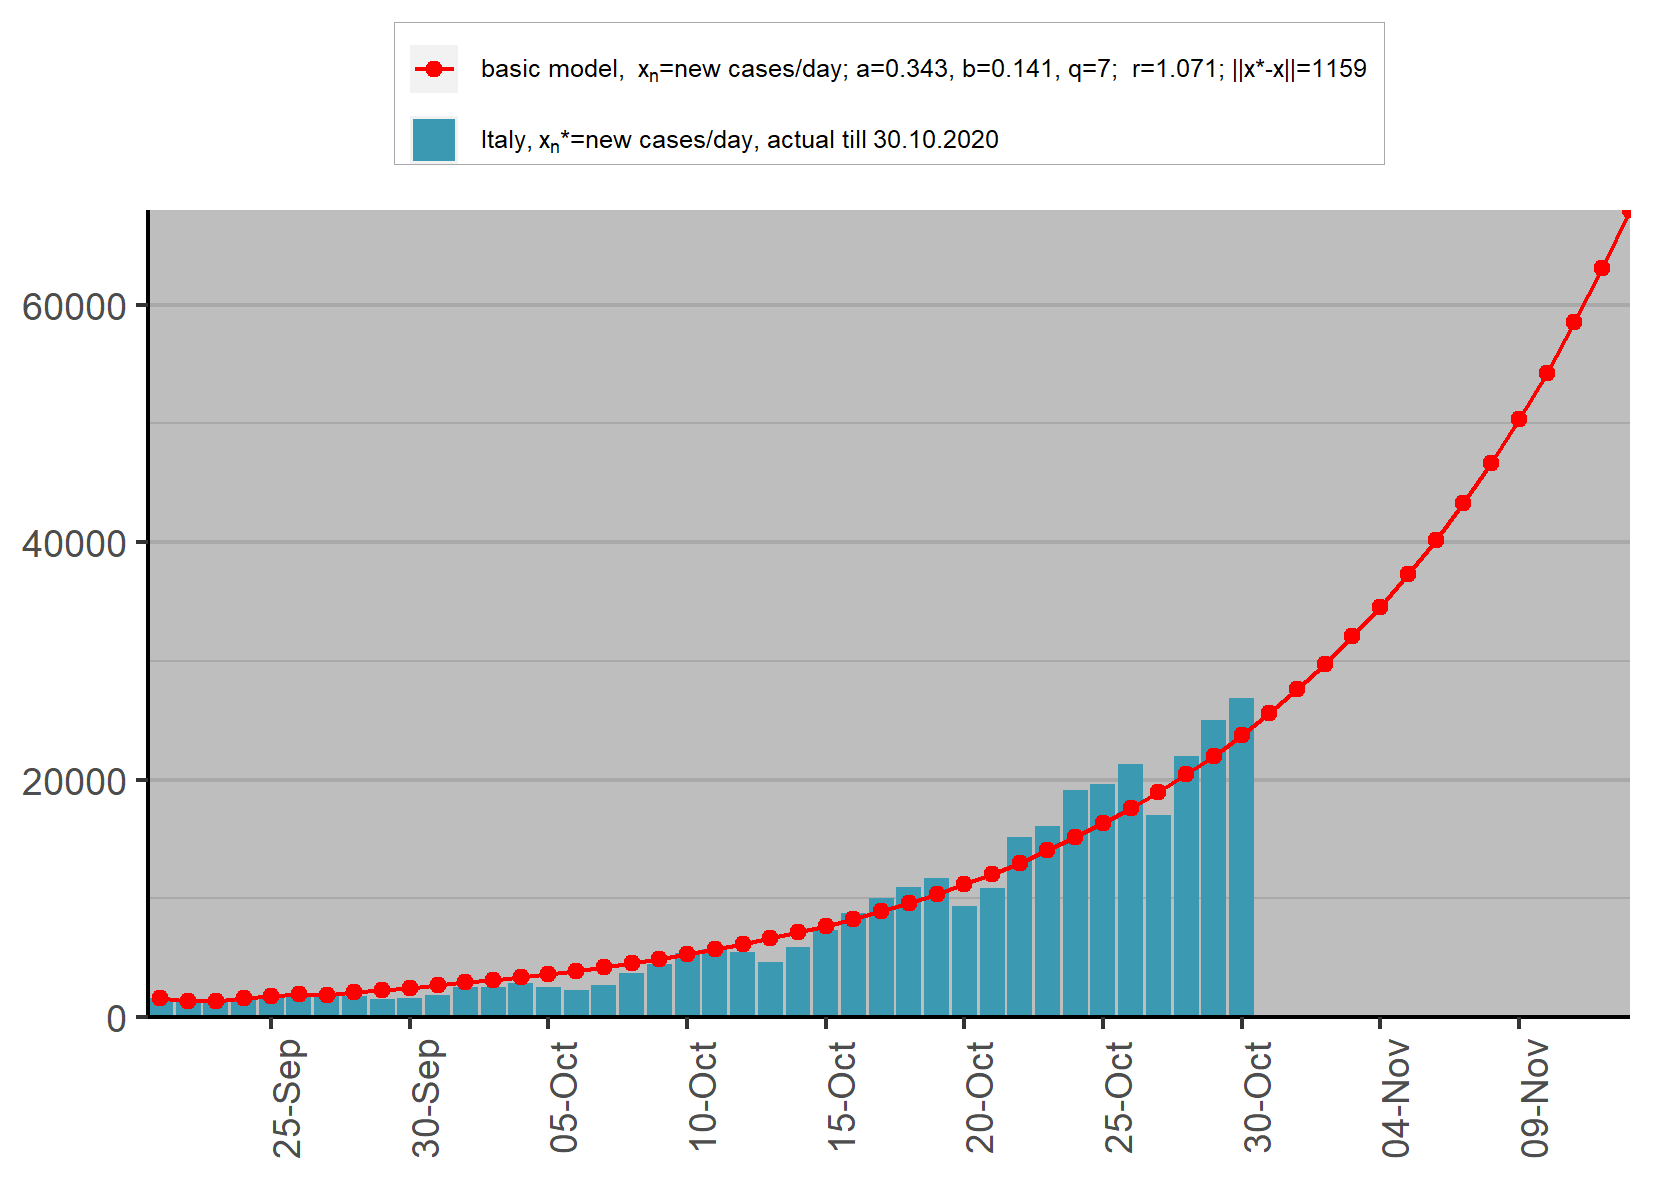
\includegraphics[width=\linewidth]{Italy-basexn.png} \label{fig:italy-basexn}
\endminipage\hfill
\minipage{0.48\textwidth}
  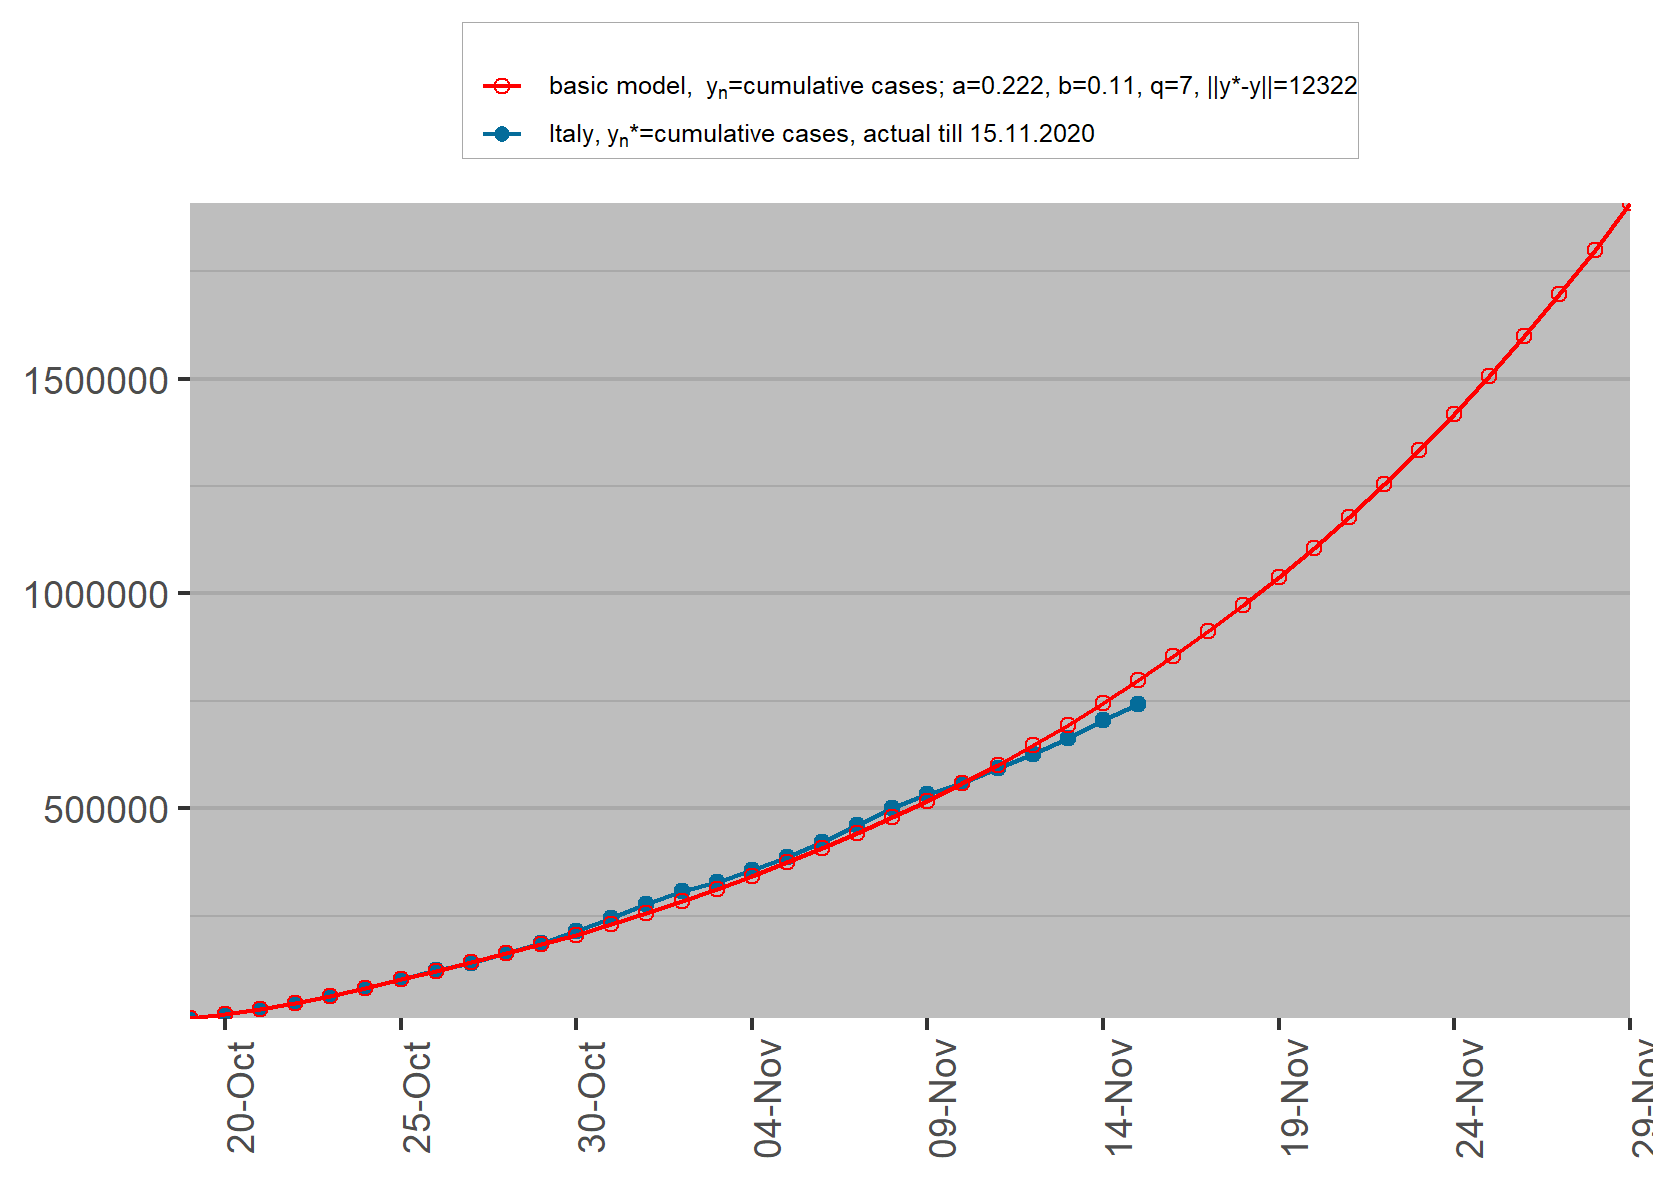
\includegraphics[width=\linewidth]{Italy-baseyn.png} \label{fig:italy-baseyn}
\endminipage
\caption{Basic model, Italy}
\end{figure}

\begin{figure}[H]
\minipage{0.48\textwidth}
  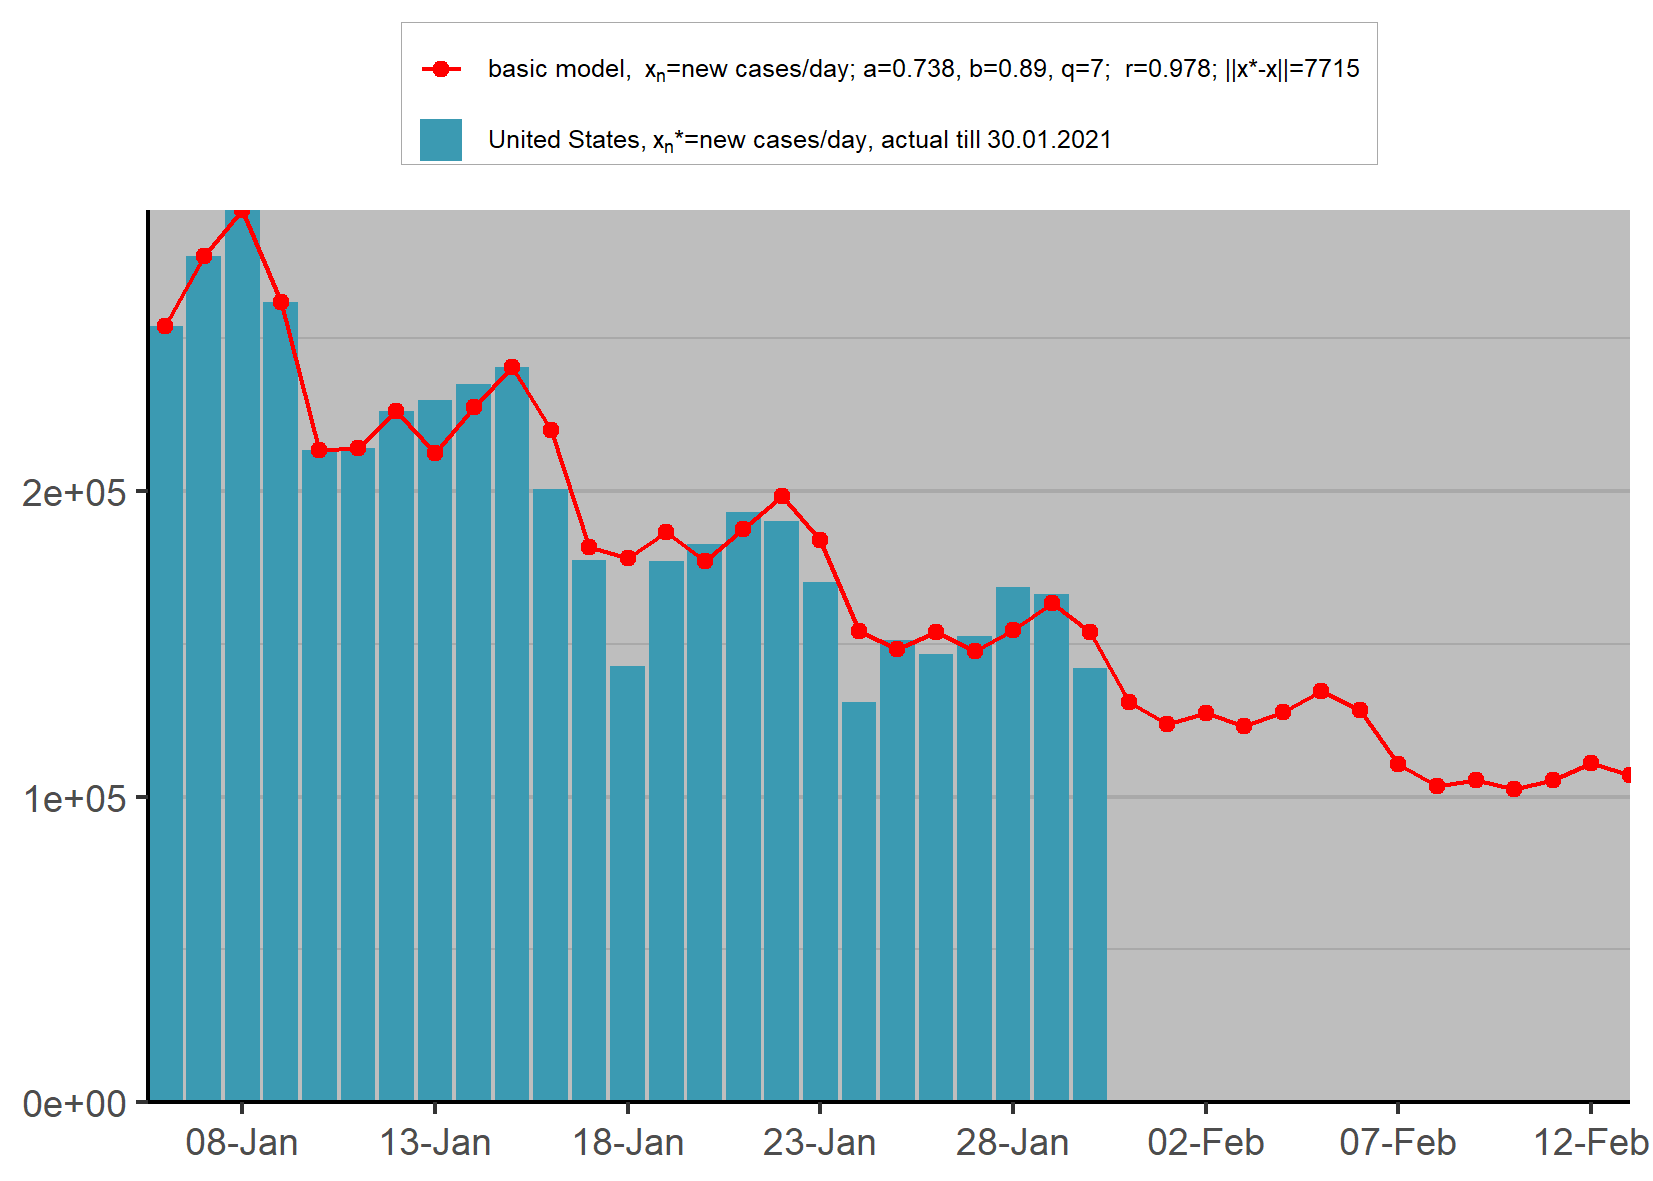
\includegraphics[width=\linewidth]{United States-basexn.png} \label{fig:usa-basexn}
\endminipage\hfill
\minipage{0.48\textwidth}
  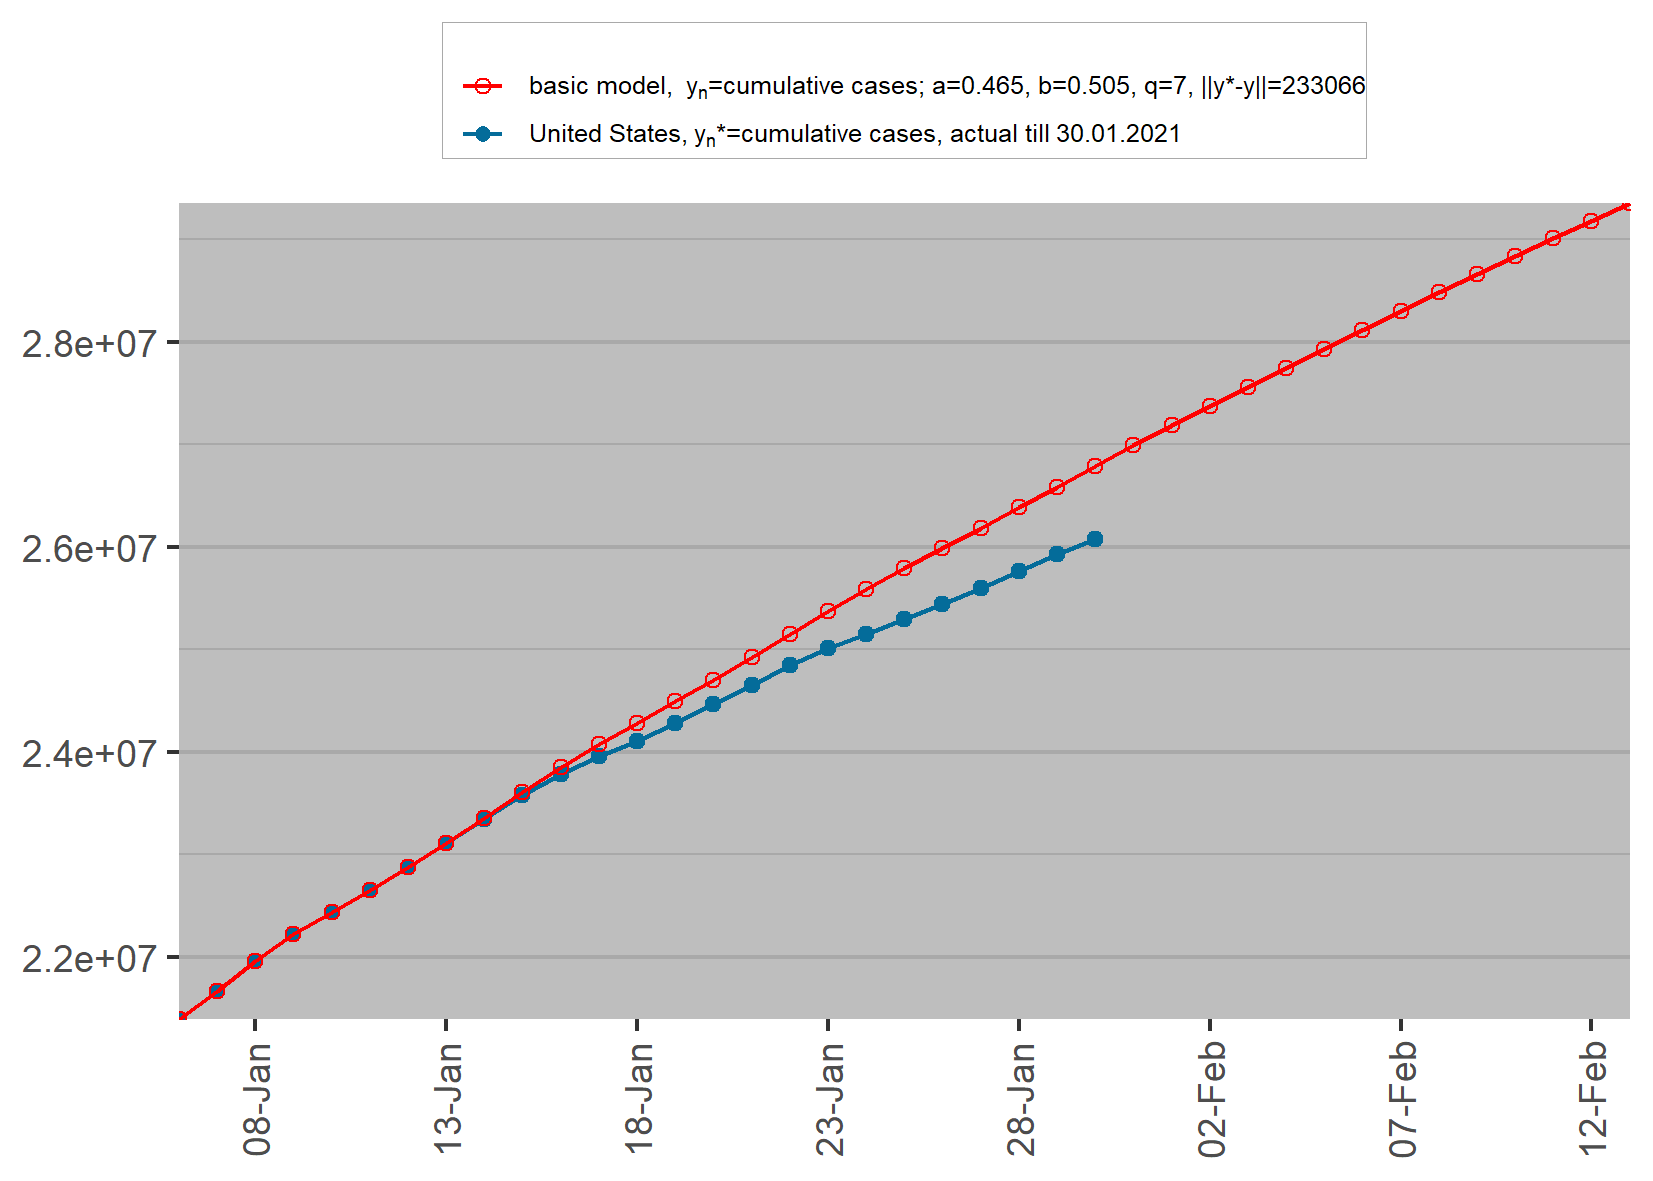
\includegraphics[width=\linewidth]{United States-baseyn.png} \label{fig:usa-baseyn}
\endminipage
\caption{Basic model, United States}
\end{figure}

\subsection{Limiting curve}

\begin{figure}[H]
\minipage{0.98\textwidth}
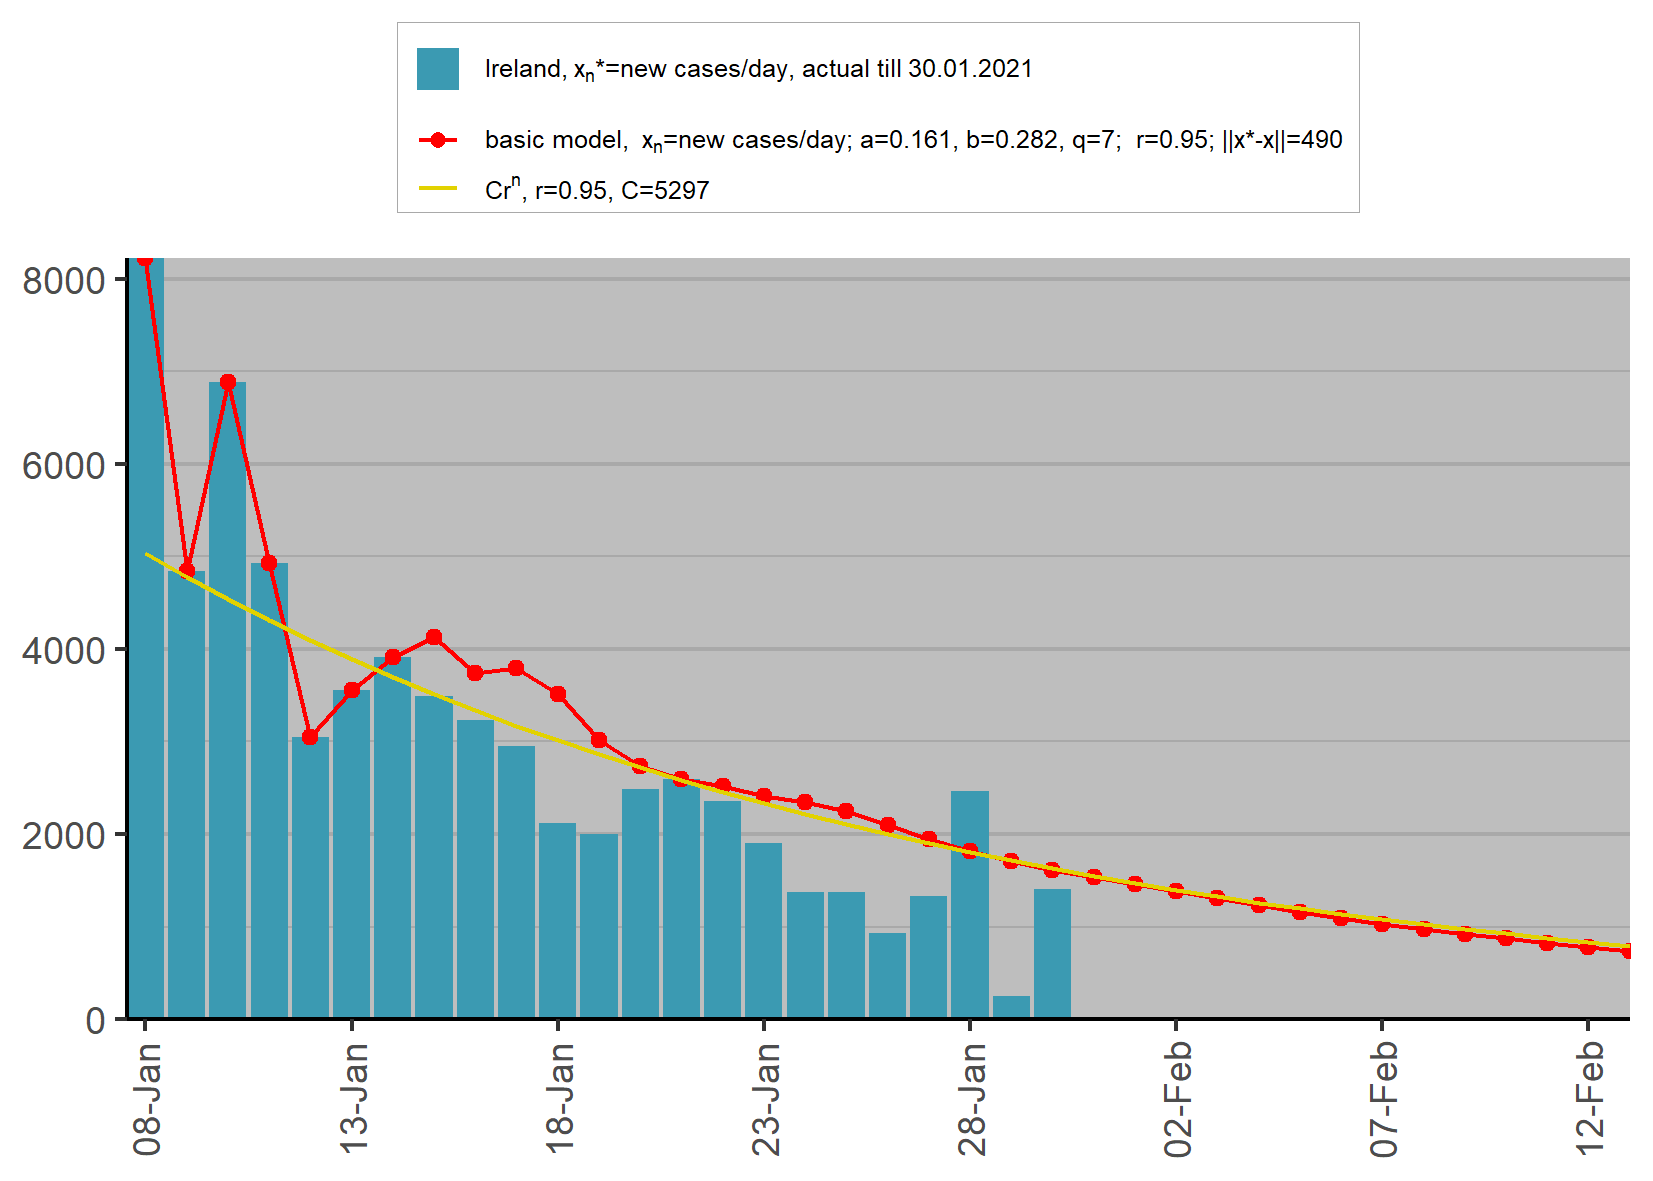
\includegraphics[width=0.9\textwidth]{Ireland-Crn.png}
\endminipage 
\caption{Comparison of $x^*_n,\ x_n$ and the limiting curve $Cr^n$, Ireland}
\end{figure}

\begin{figure}[H]
\minipage{0.98\textwidth}
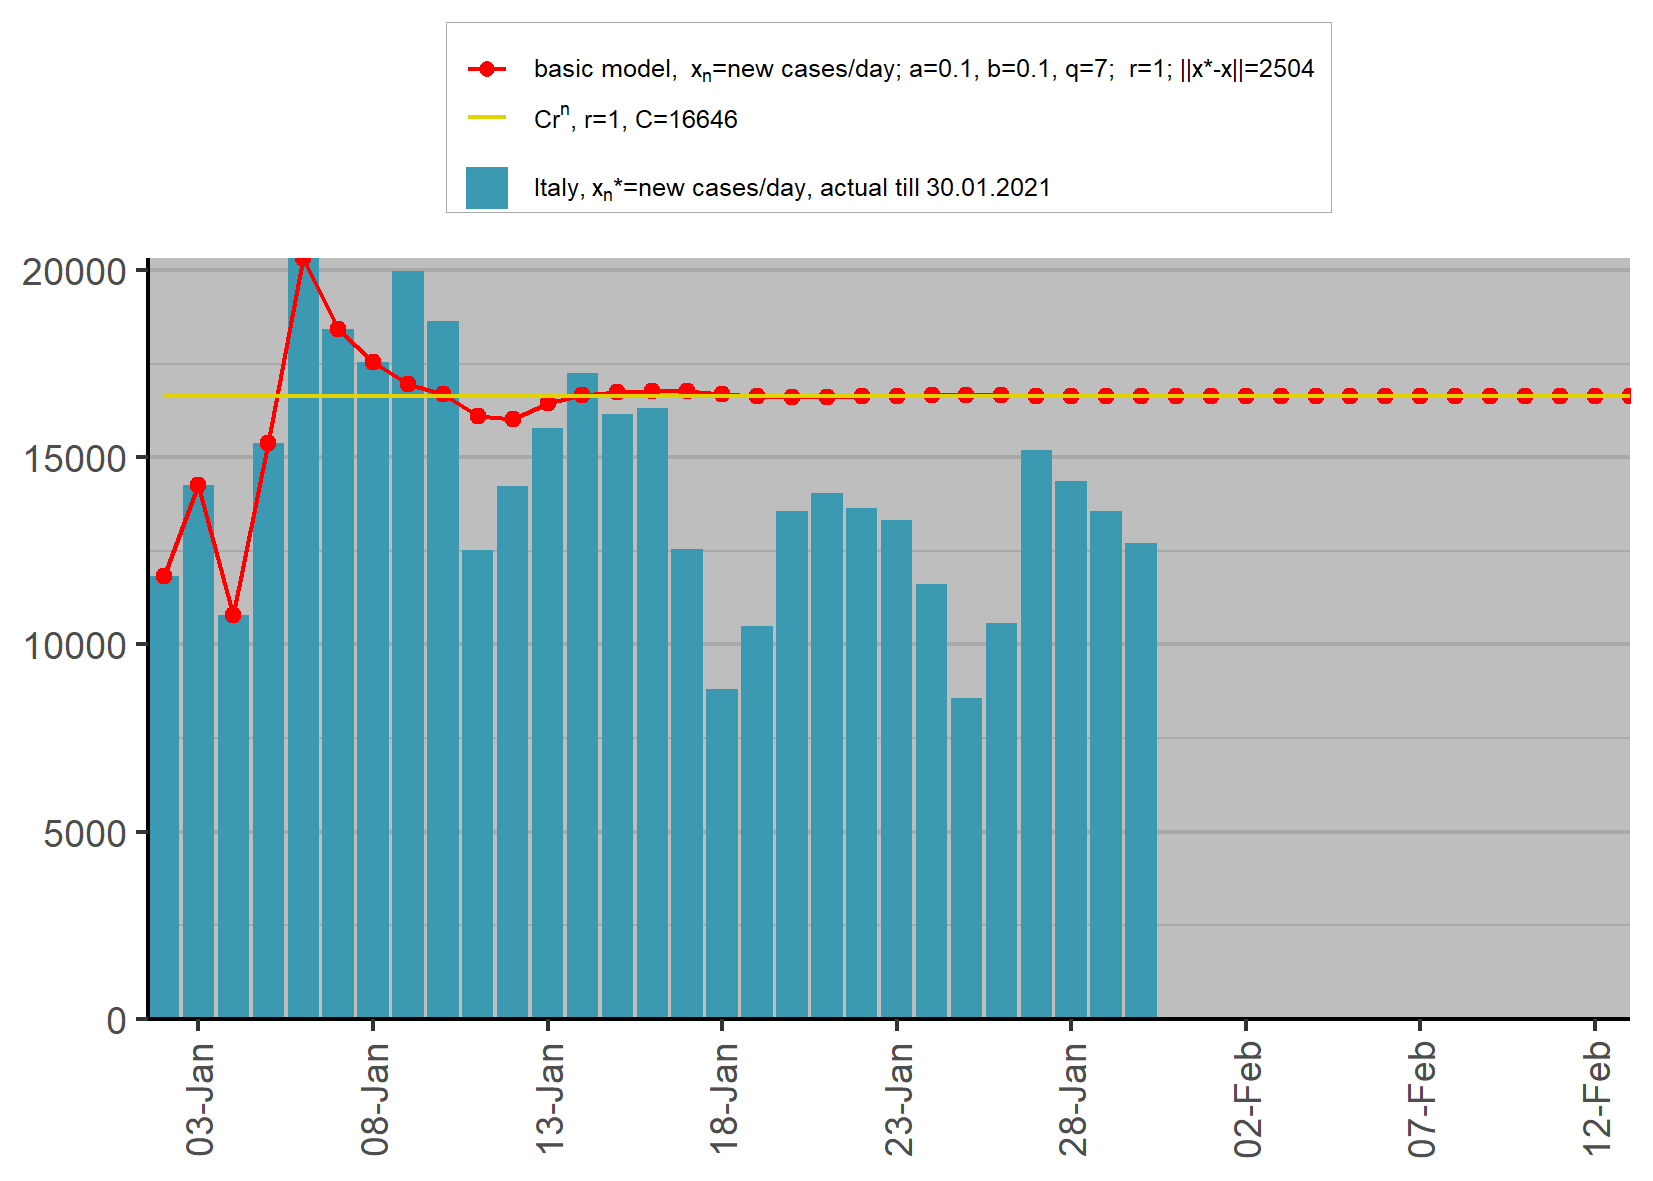
\includegraphics[width=0.9\textwidth]{Italy-Crn.png}
\endminipage 
\caption{Comparison of $x^*_n,\ x_n$ and the limiting curve $Cr^n$, Italy}
\end{figure}

\begin{figure}[H]
\minipage{0.98\textwidth}
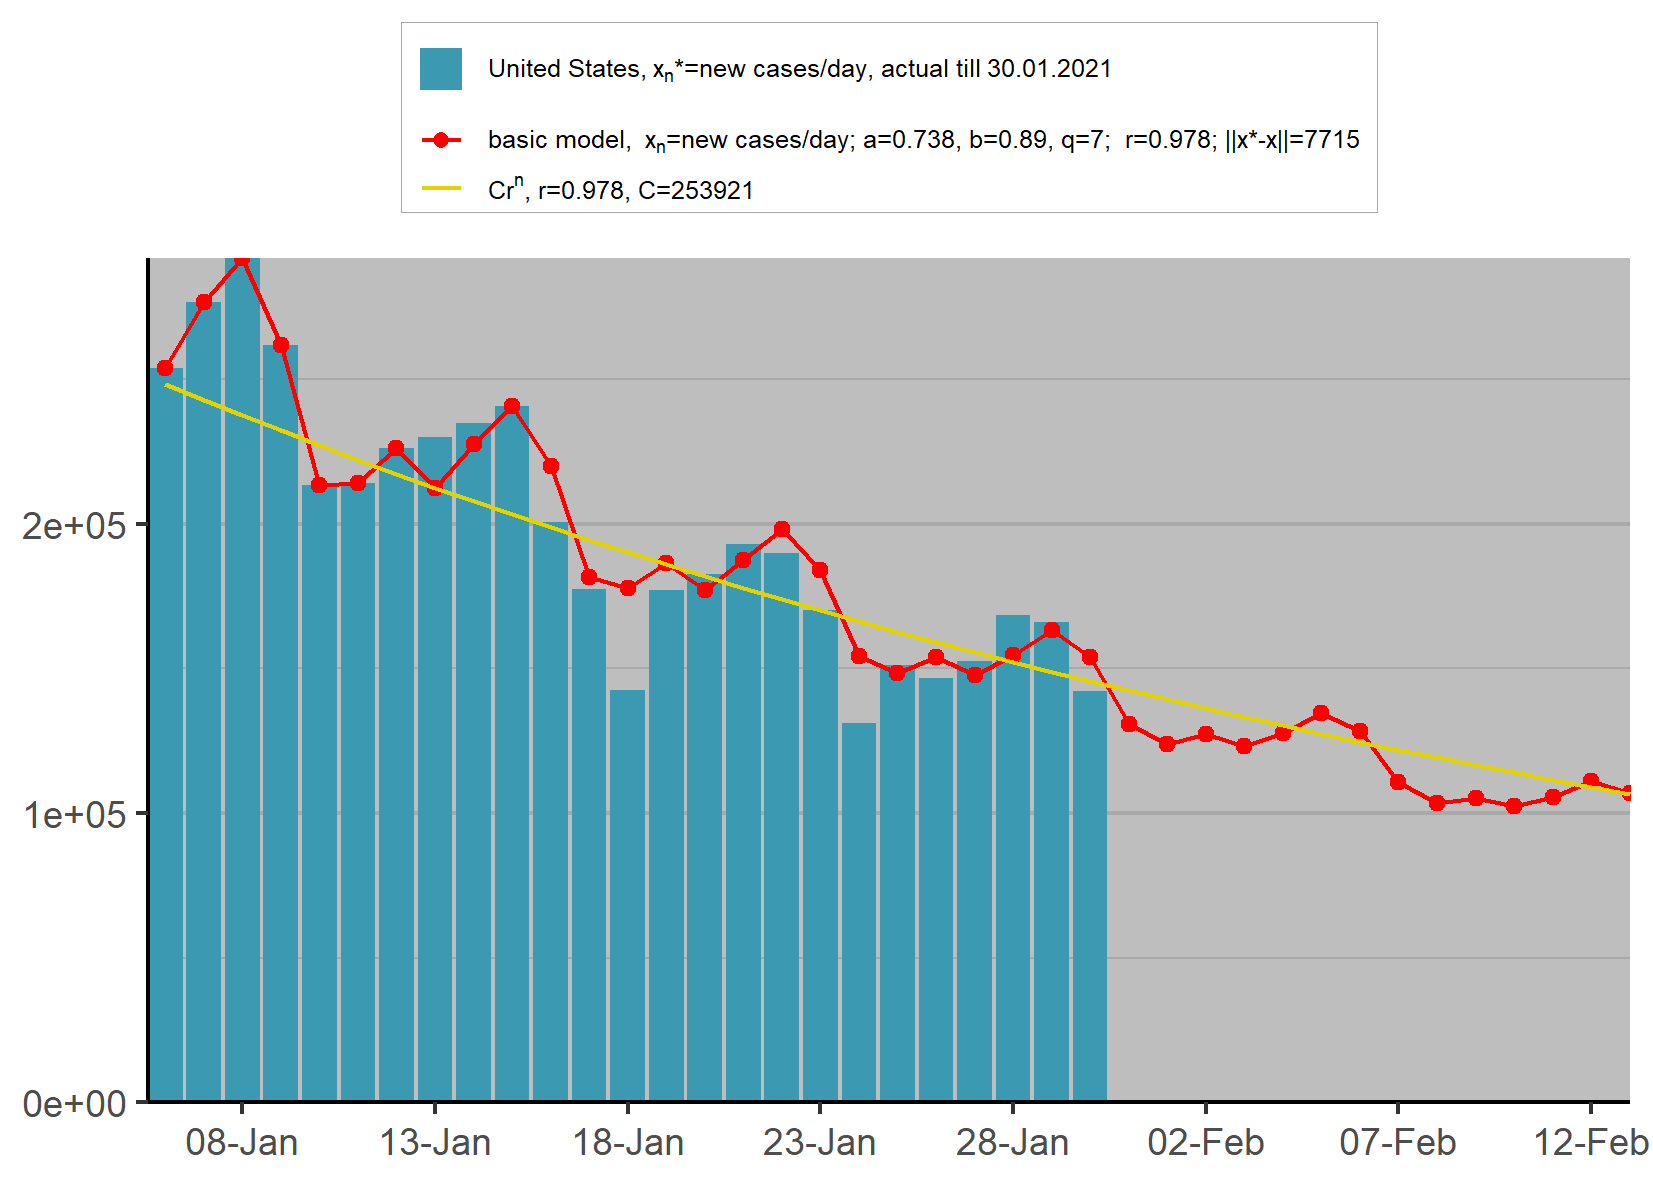
\includegraphics[width=0.9\textwidth]{United States-Crn.png}
\endminipage 
\caption{Comparison of $x^*_n,\ x_n$ and the limiting curve $Cr^n$, United States}
\end{figure}

\subsection{Moving average}

\begin{figure}[H]
\minipage{0.98\textwidth}
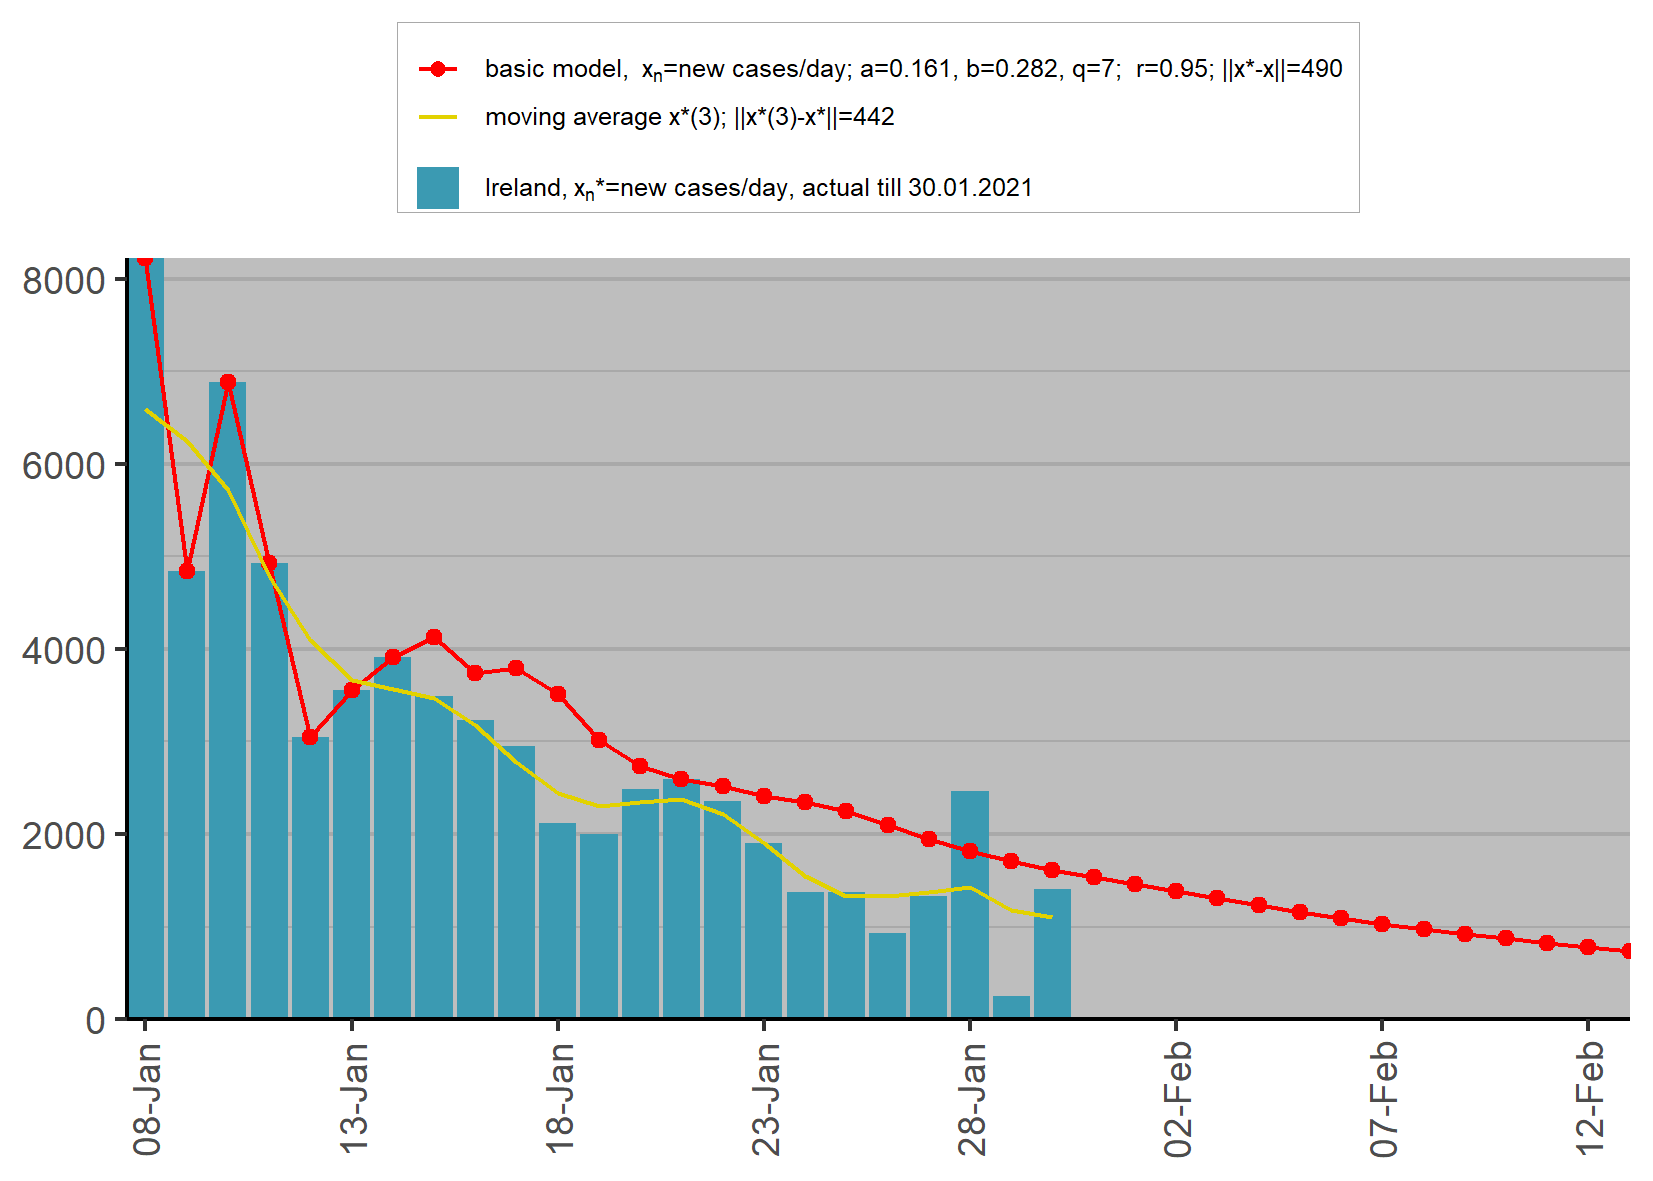
\includegraphics[width=0.9\textwidth]{Ireland-mavgx3.png}
\endminipage 
\caption{Moving average $x^*_n (3)$, Ireland}
\end{figure}

\begin{figure}[H]
\minipage{0.98\textwidth}
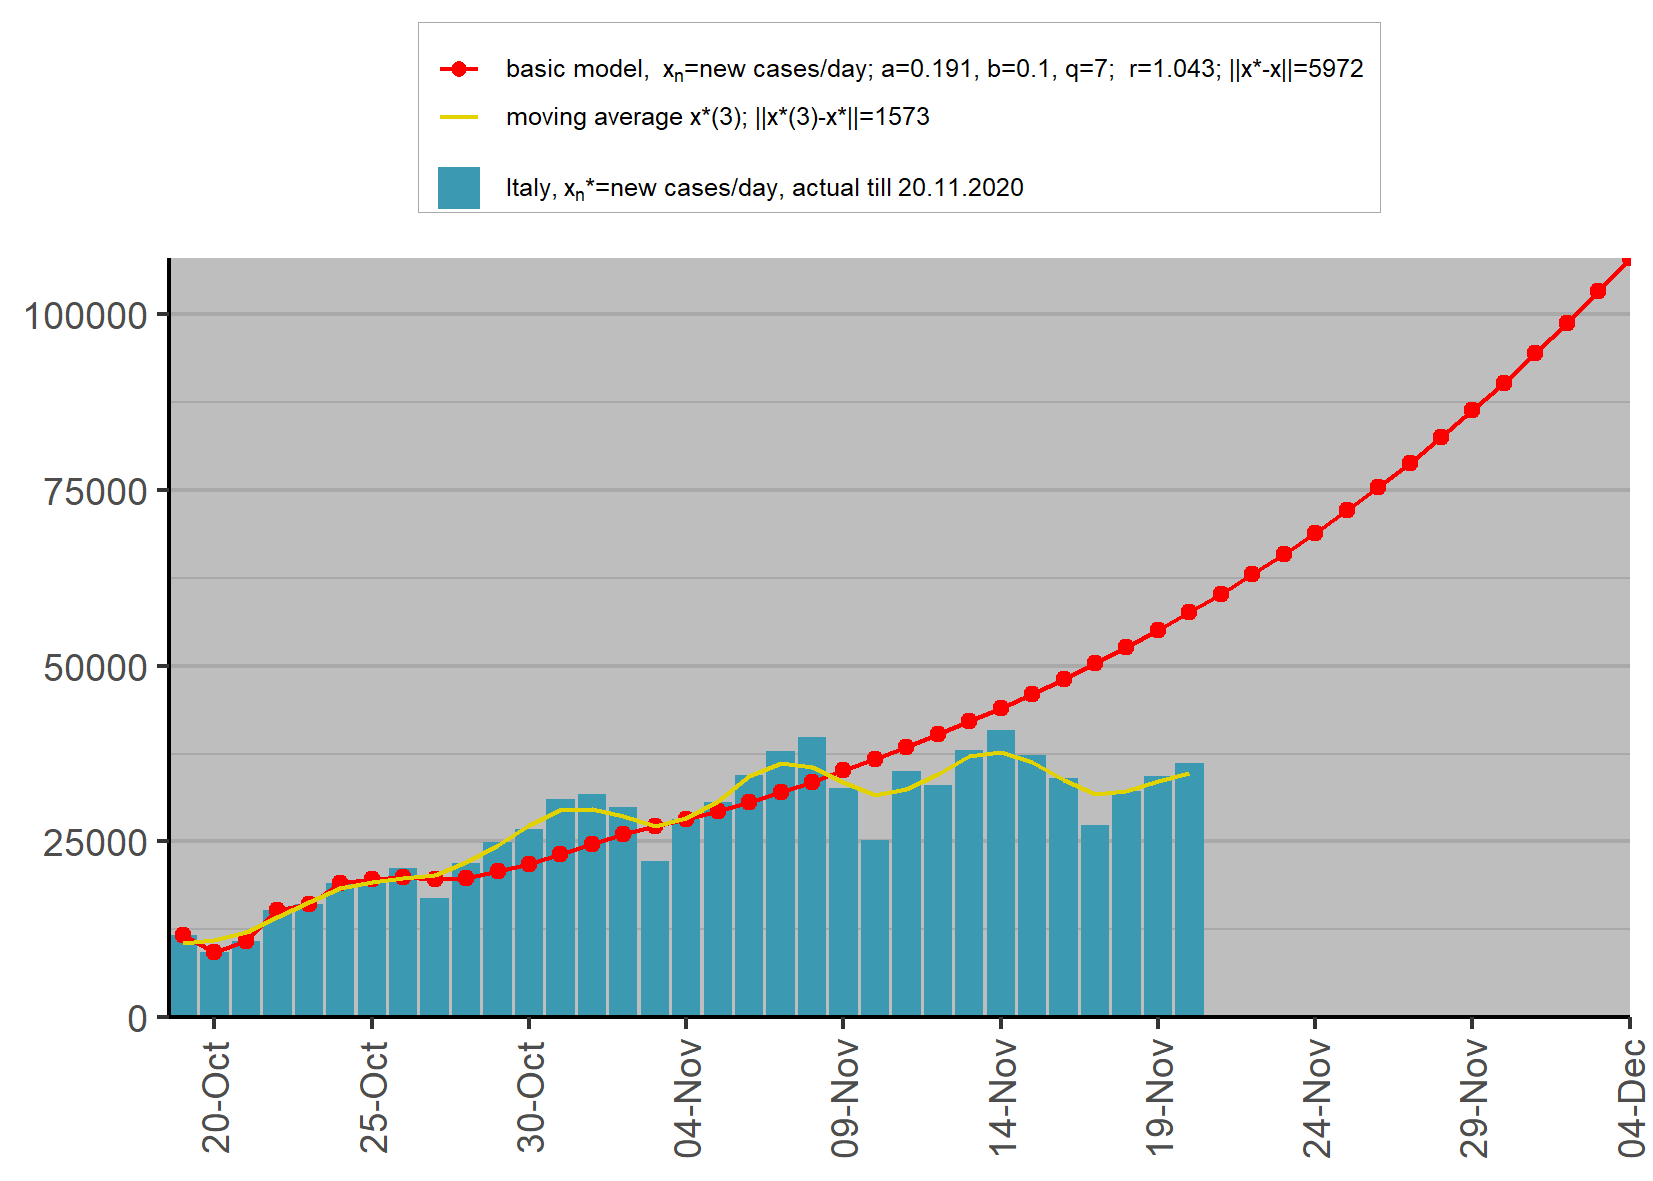
\includegraphics[width=0.9\textwidth]{Italy-mavgx3.png}
\endminipage 
\caption{Moving average $x^*_n (3)$, Italy}
\end{figure}

\begin{figure}[H]
\minipage{0.98\textwidth}
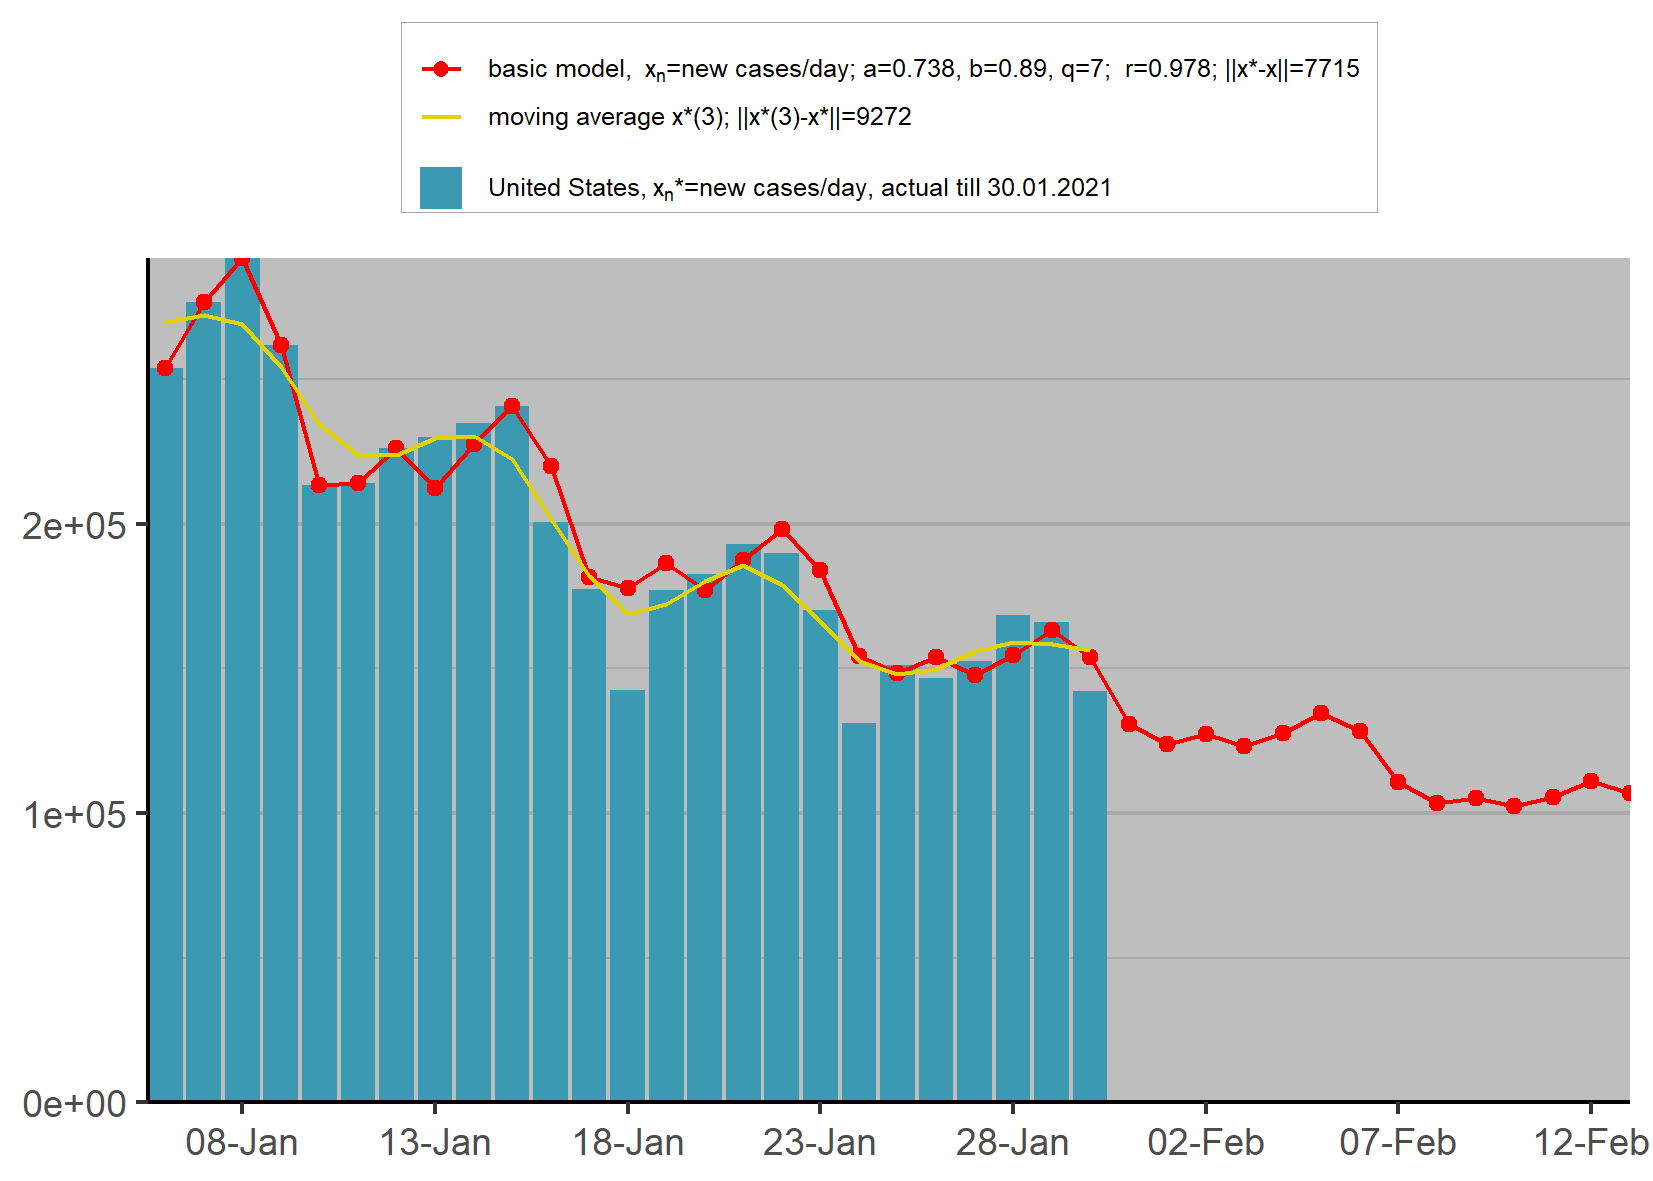
\includegraphics[width=0.9\textwidth]{United States-mavgx3.png}
\endminipage 
\caption{Moving average $x^*_n (3)$, United States}
\end{figure}

\subsection{Periodic model}

\subsubsection{Definitions and Theory}

\subsubsection{How to select the best model}

\subsubsection{Forecasting}

\subsubsection{Implementation in R}

\begin{figure}[H]
\minipage{0.98\textwidth}
  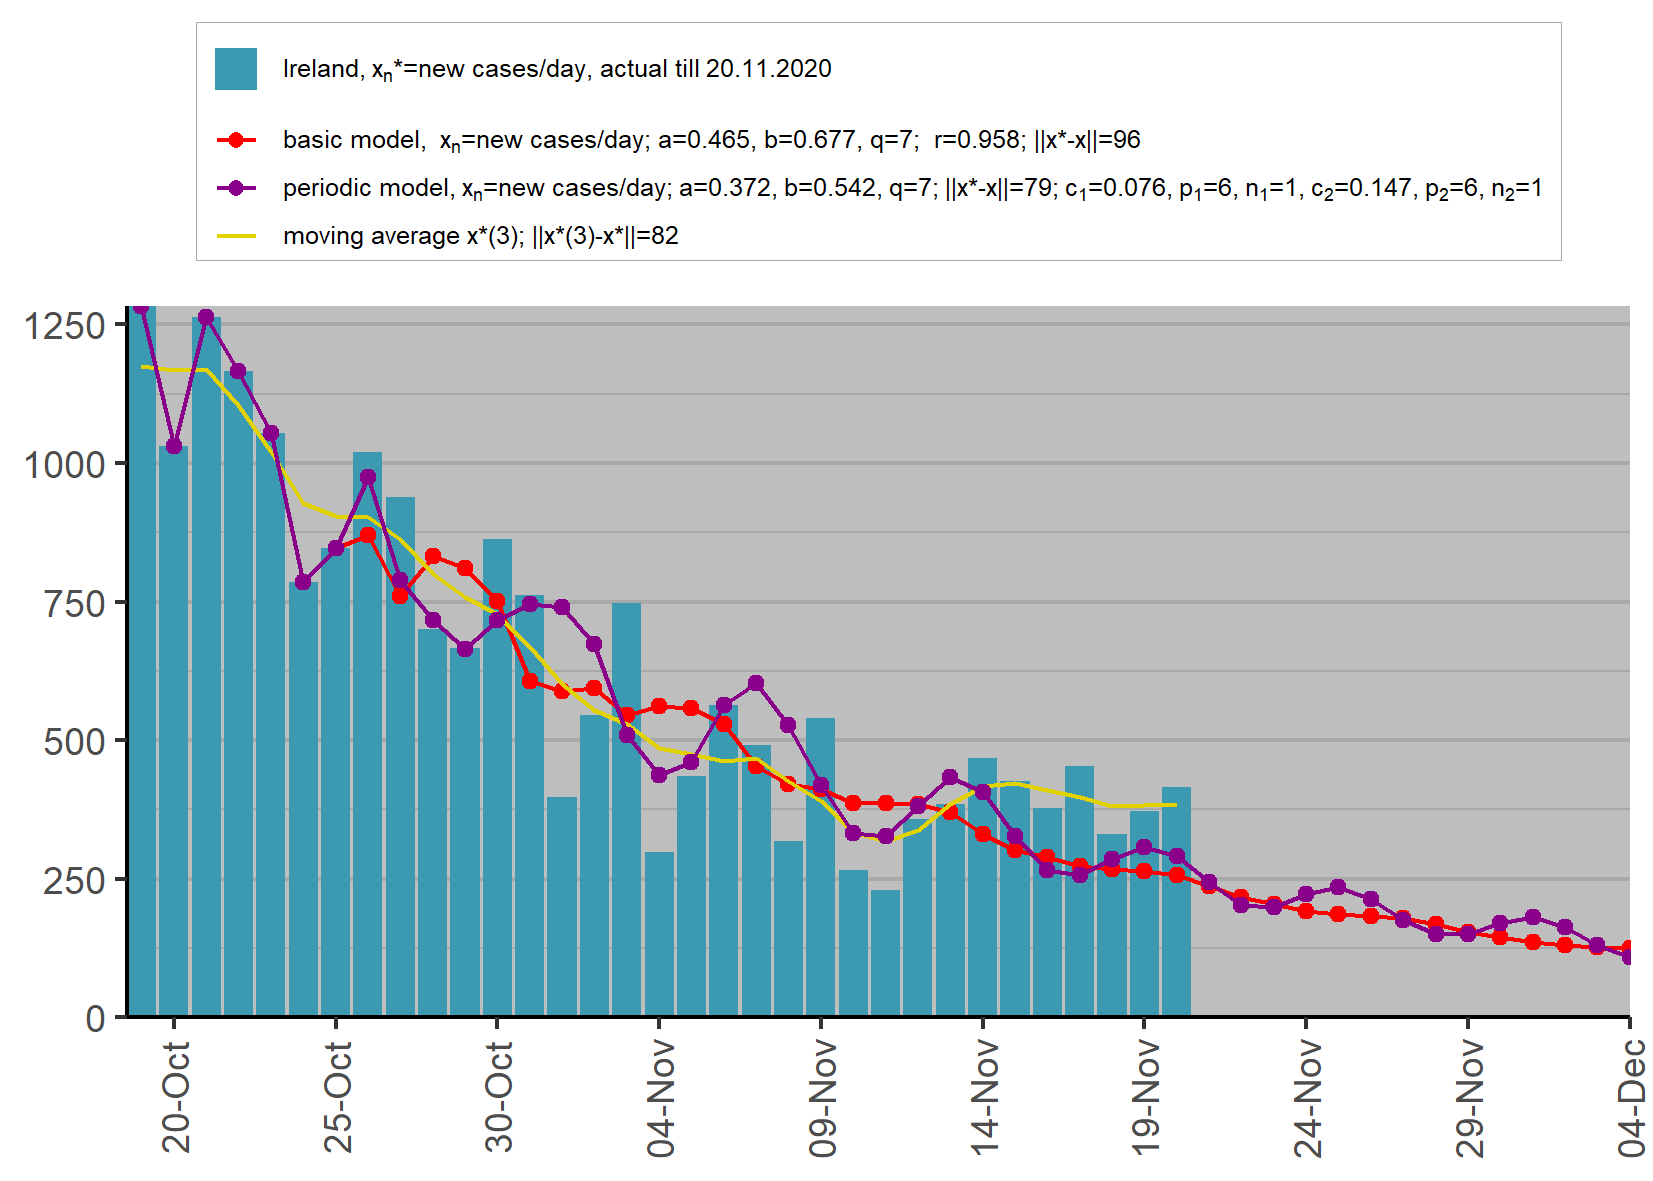
\includegraphics[width=\linewidth]{Ireland-periodic.png} \label{fig:usa-periodic}
\endminipage
\caption{Periodic Model, Ireland}
\end{figure}

\begin{figure}[H]
\minipage{0.98\textwidth}
  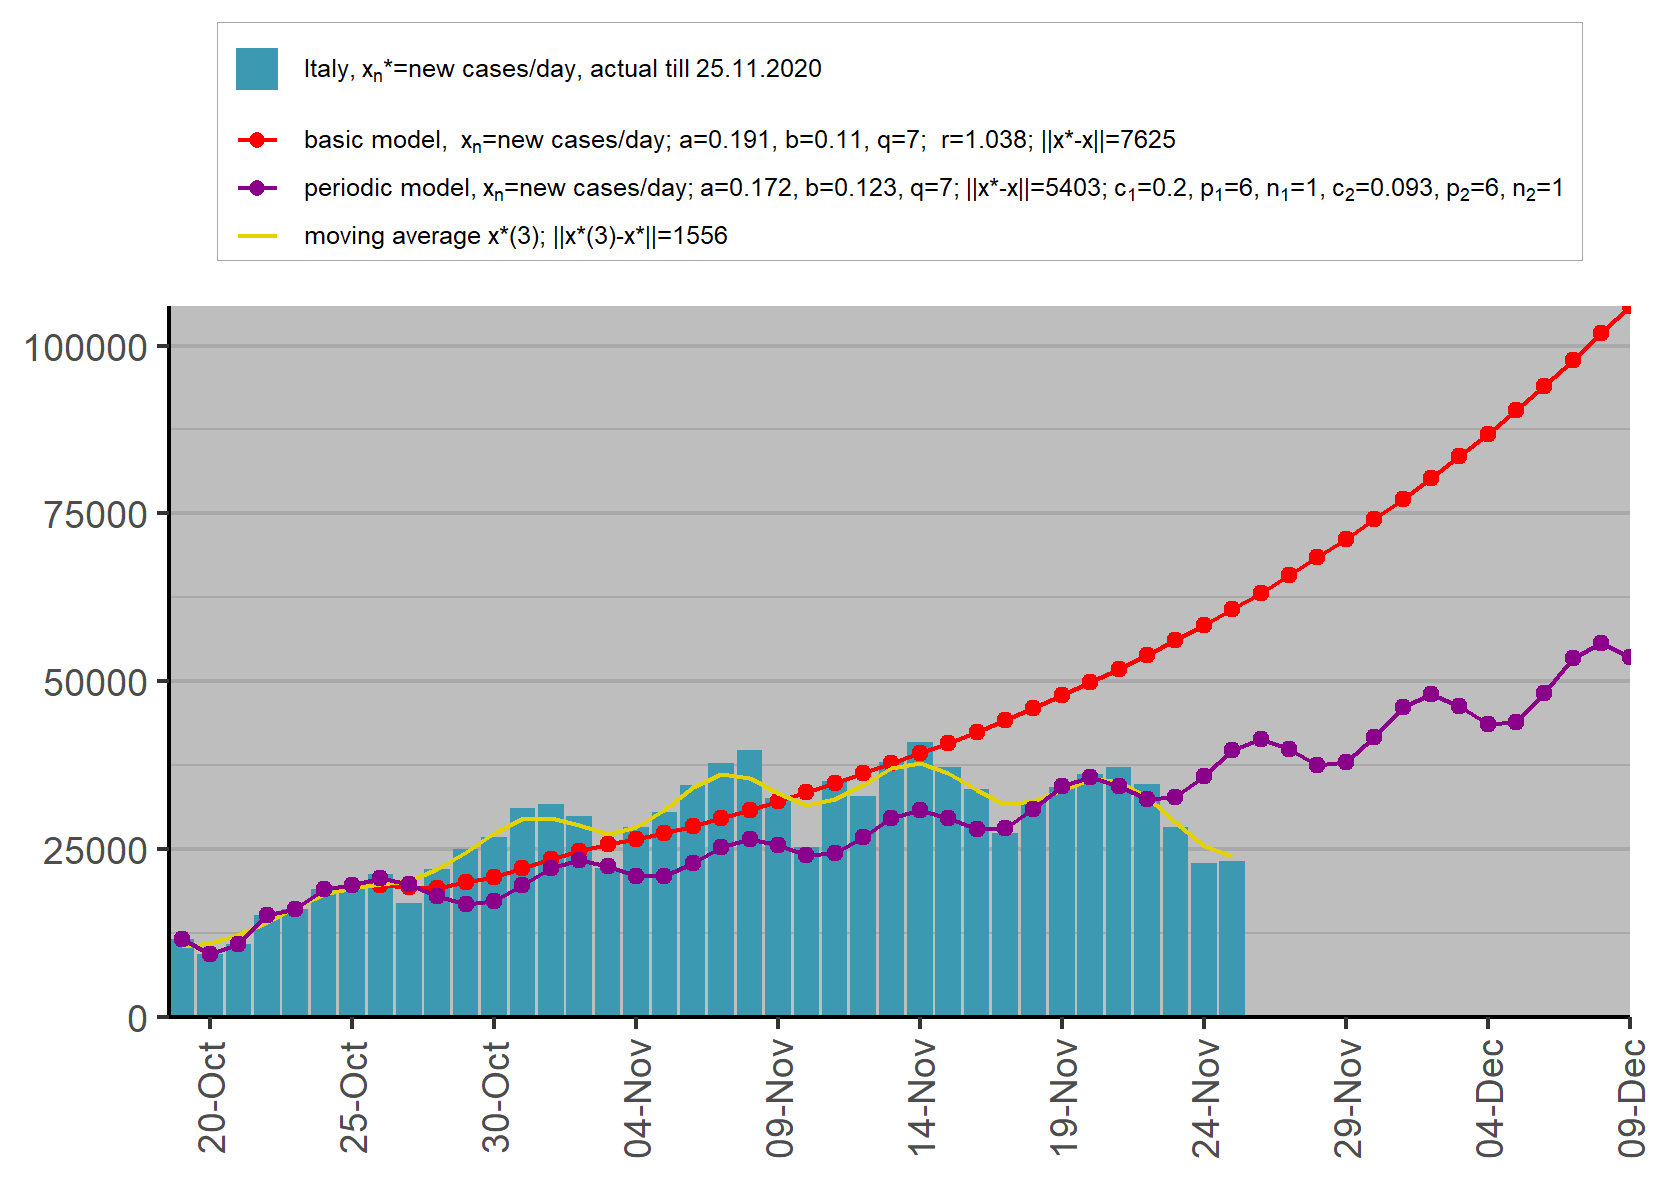
\includegraphics[width=\linewidth]{Italy-periodic.png} \label{fig:italy-periodic}
\endminipage 
\caption{Periodic Model, Italy}
\end{figure}

\begin{figure}[H]
\minipage{0.98\textwidth}
  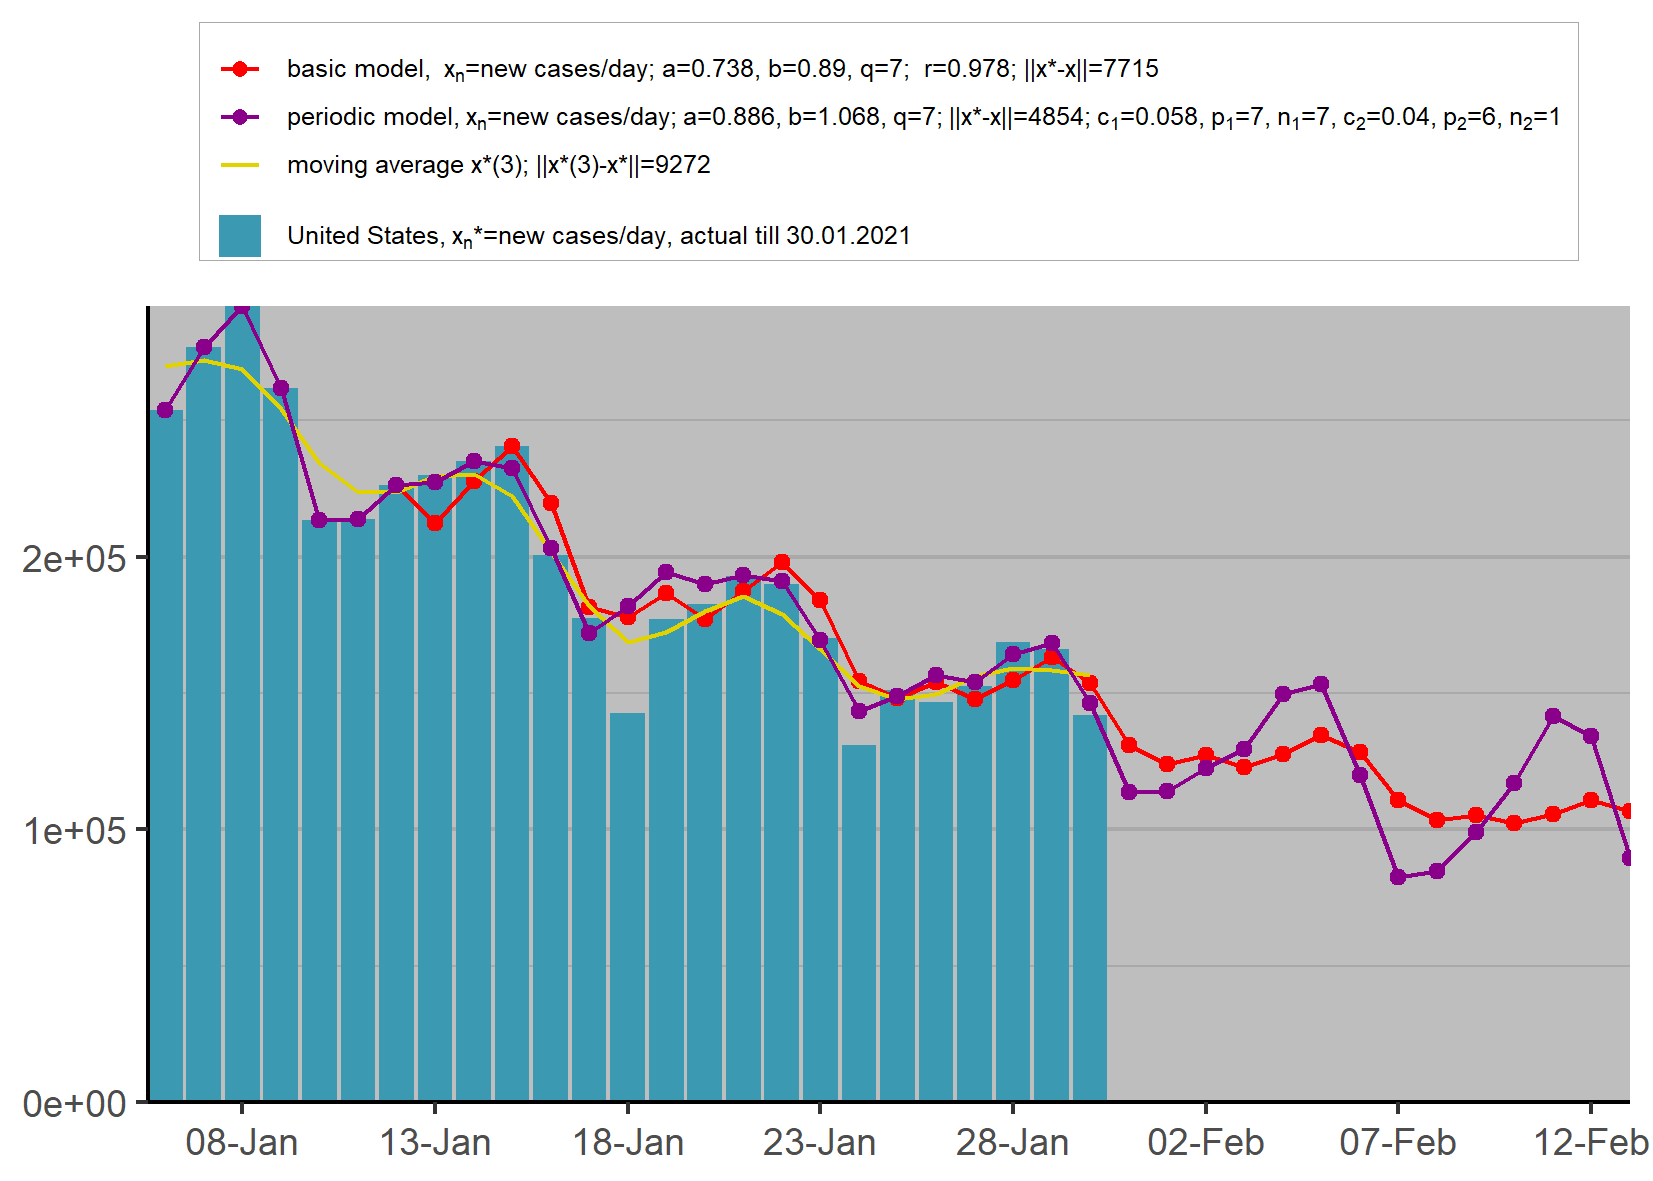
\includegraphics[width=\linewidth]{United States-periodic.png} \label{fig:usa-periodic}
\endminipage
\caption{Periodic Model, Ireland}
\end{figure}

\subsection{Multi-phase model}

\subsubsection{Definitions and Theory}

\subsubsection{How to select the best model}

\subsubsection{Forecasting}

\subsubsection{Implementation in R}

The multi-phase model without periodicity can be sharp and unrealstic

\begin{figure}[H]
\minipage{0.48\textwidth}
  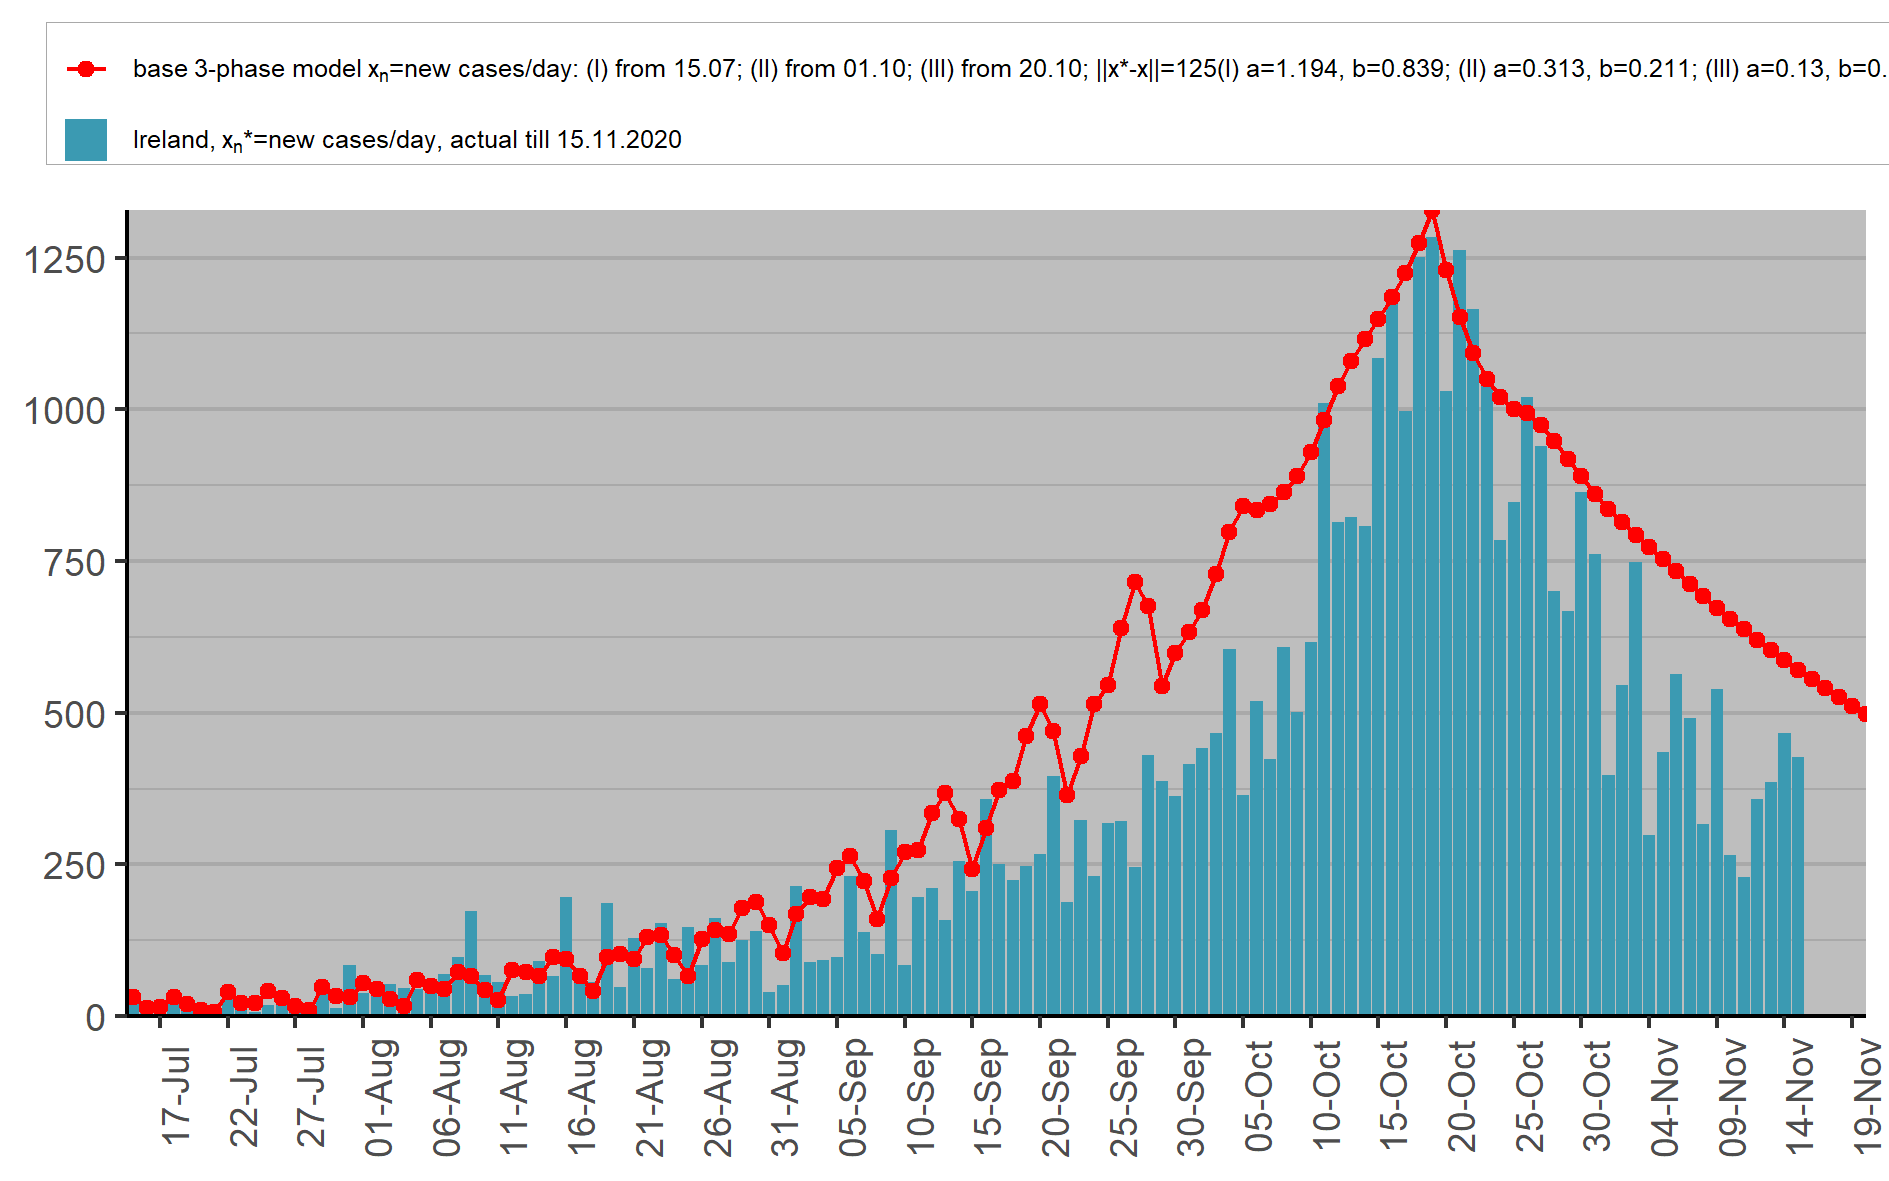
\includegraphics[width=\linewidth]{Ireland-xnmult.png} \label{fig:ireland-xnmult}
\endminipage\hfill
\minipage{0.48\textwidth}
  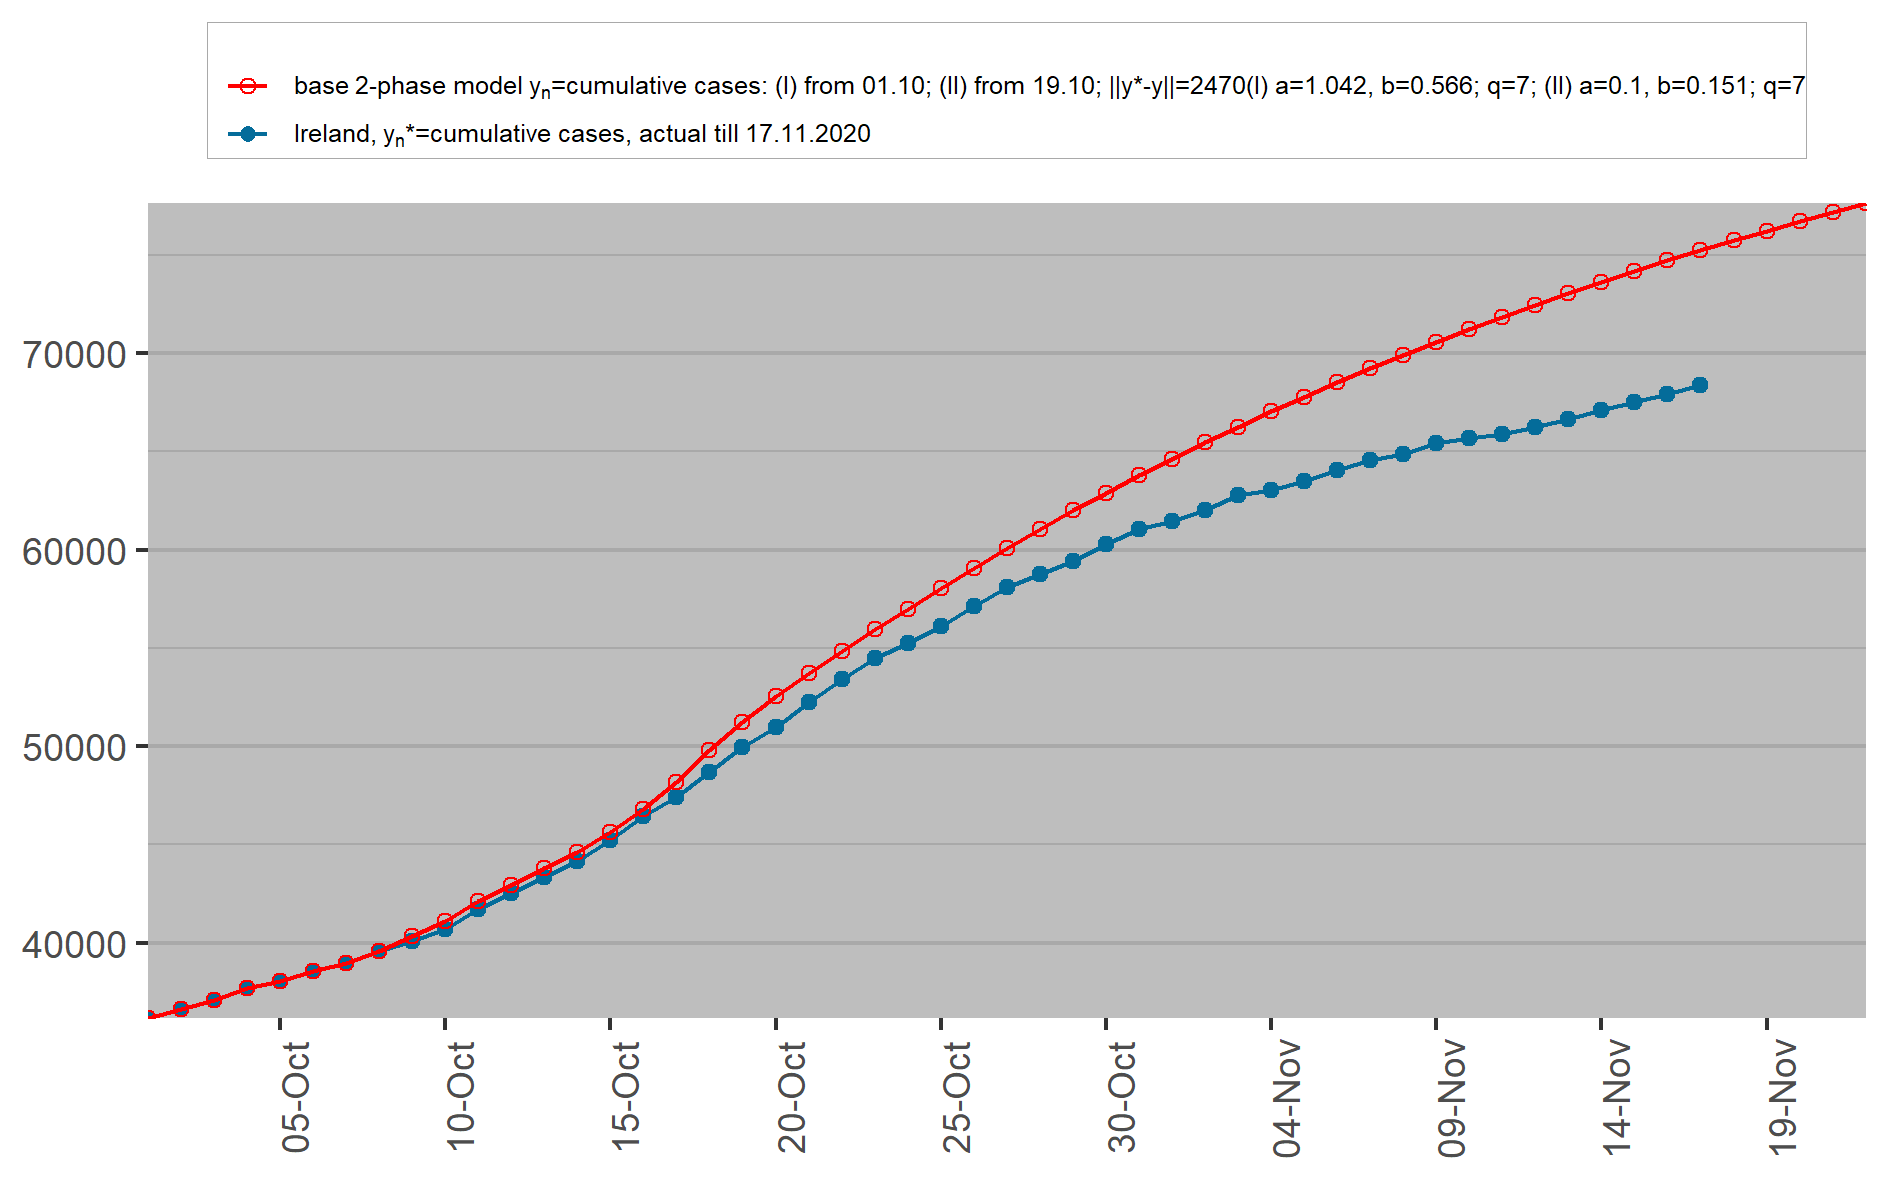
\includegraphics[width=\linewidth]{Ireland-ynmult.png} \label{fig:ireland-ynmult}
\endminipage
\caption{Multi-phase model, Ireland}
\end{figure}

\begin{figure}[H]
\minipage{0.48\textwidth}
  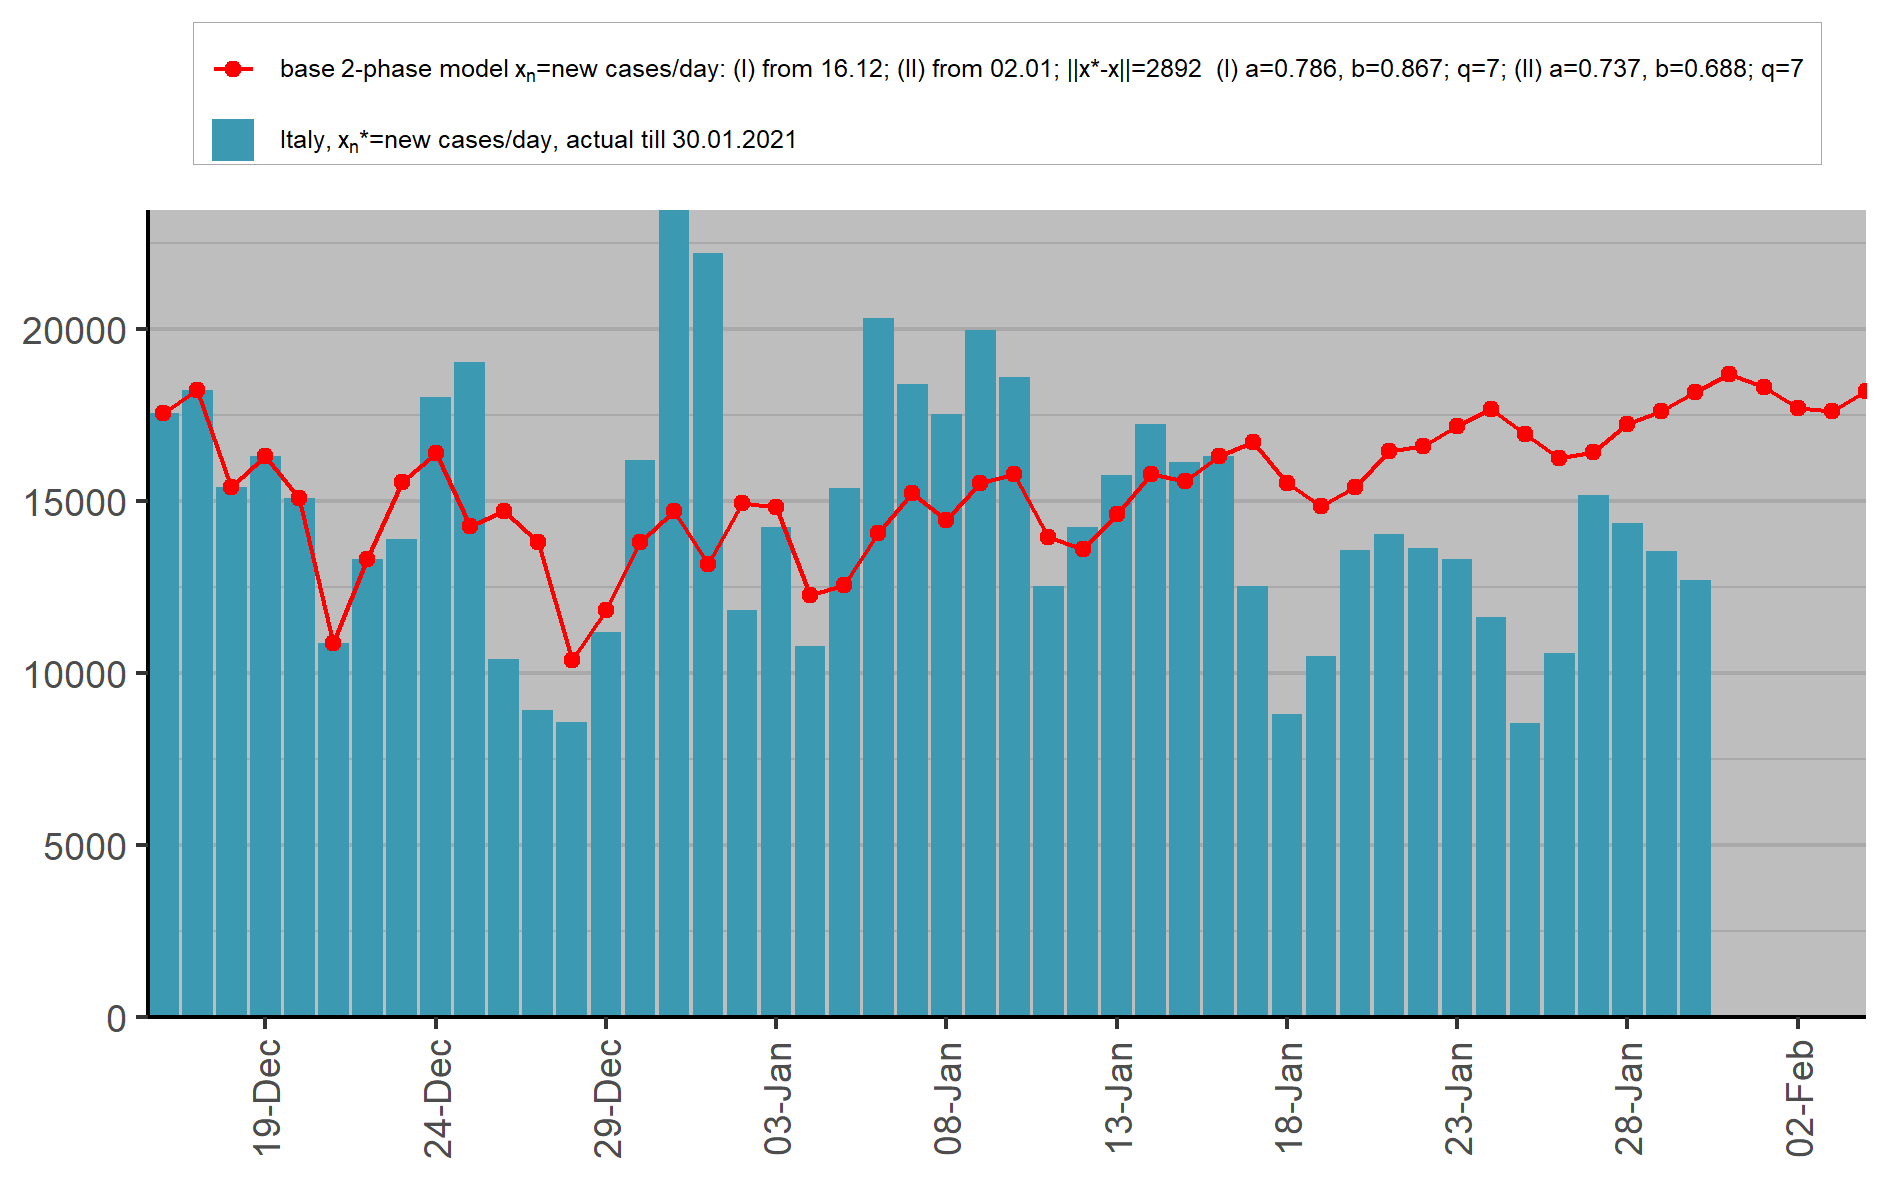
\includegraphics[width=\linewidth]{Italy-xnmult.png} \label{fig:italy-xnmult}
\endminipage\hfill
\minipage{0.48\textwidth}
  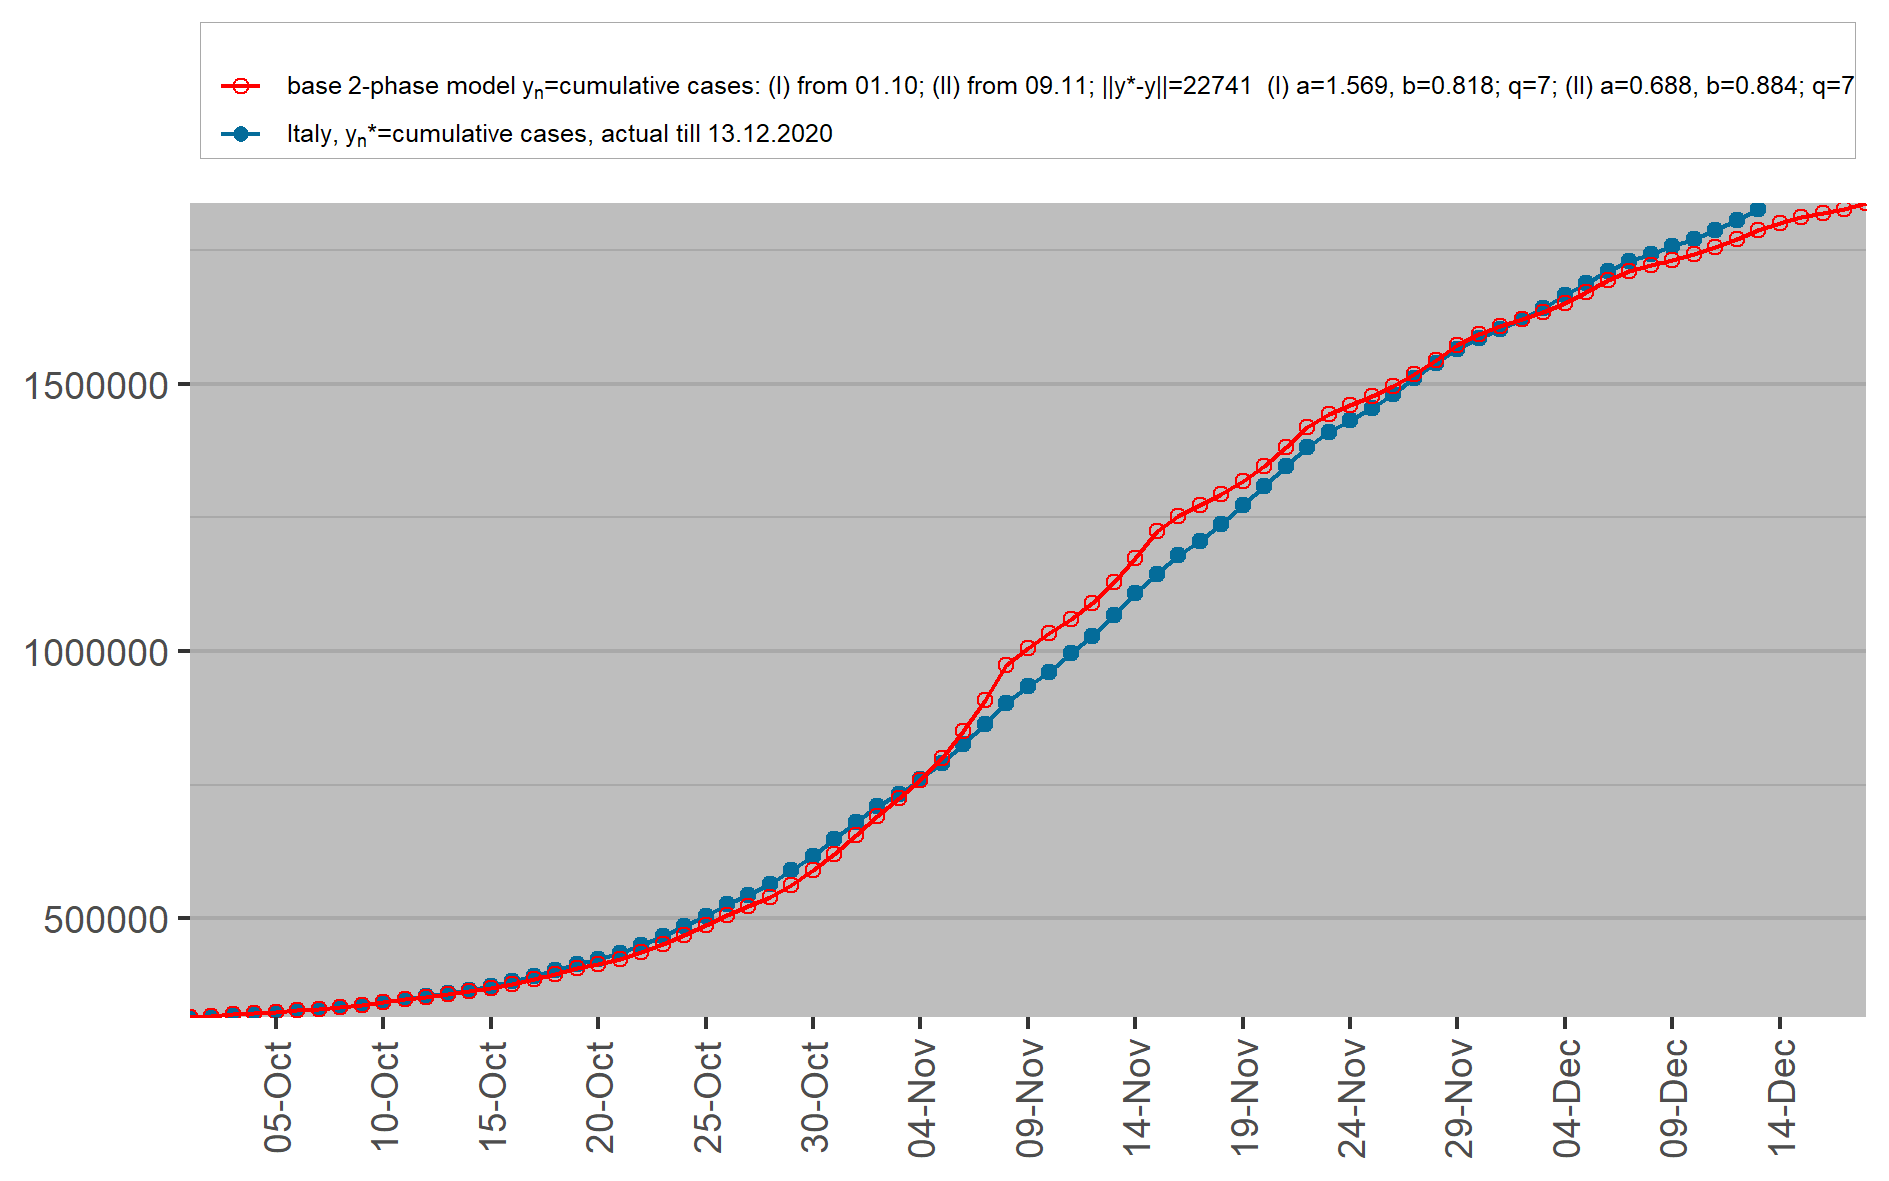
\includegraphics[width=\linewidth]{Italy-ynmult.png} \label{fig:italy-ynmult}
\endminipage
\caption{Multi-phase model, Italy}
\end{figure}

\begin{figure}[H]
\minipage{0.48\textwidth}
  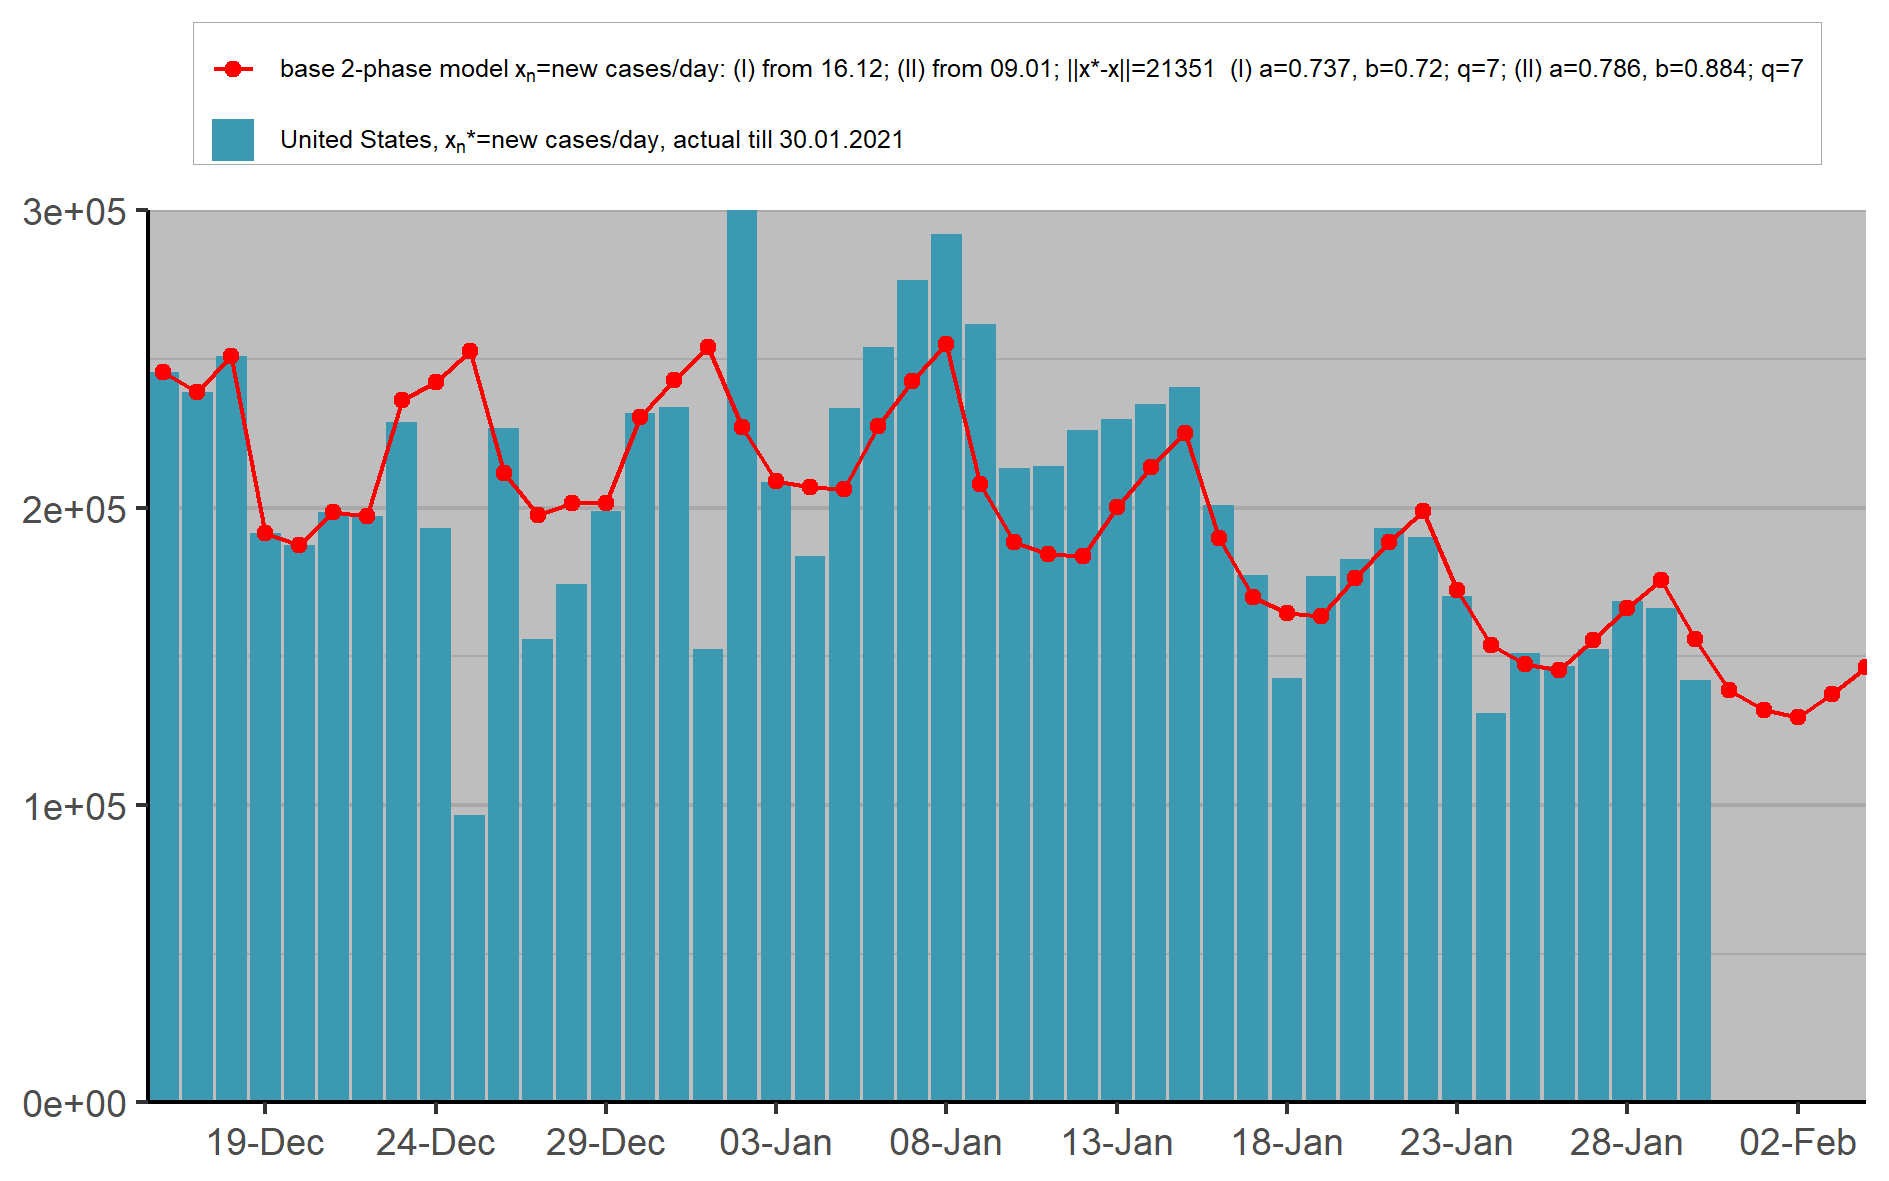
\includegraphics[width=\linewidth]{United States-xnmult.png} \label{fig:usa-xnmult}
\endminipage\hfill
\minipage{0.48\textwidth}
  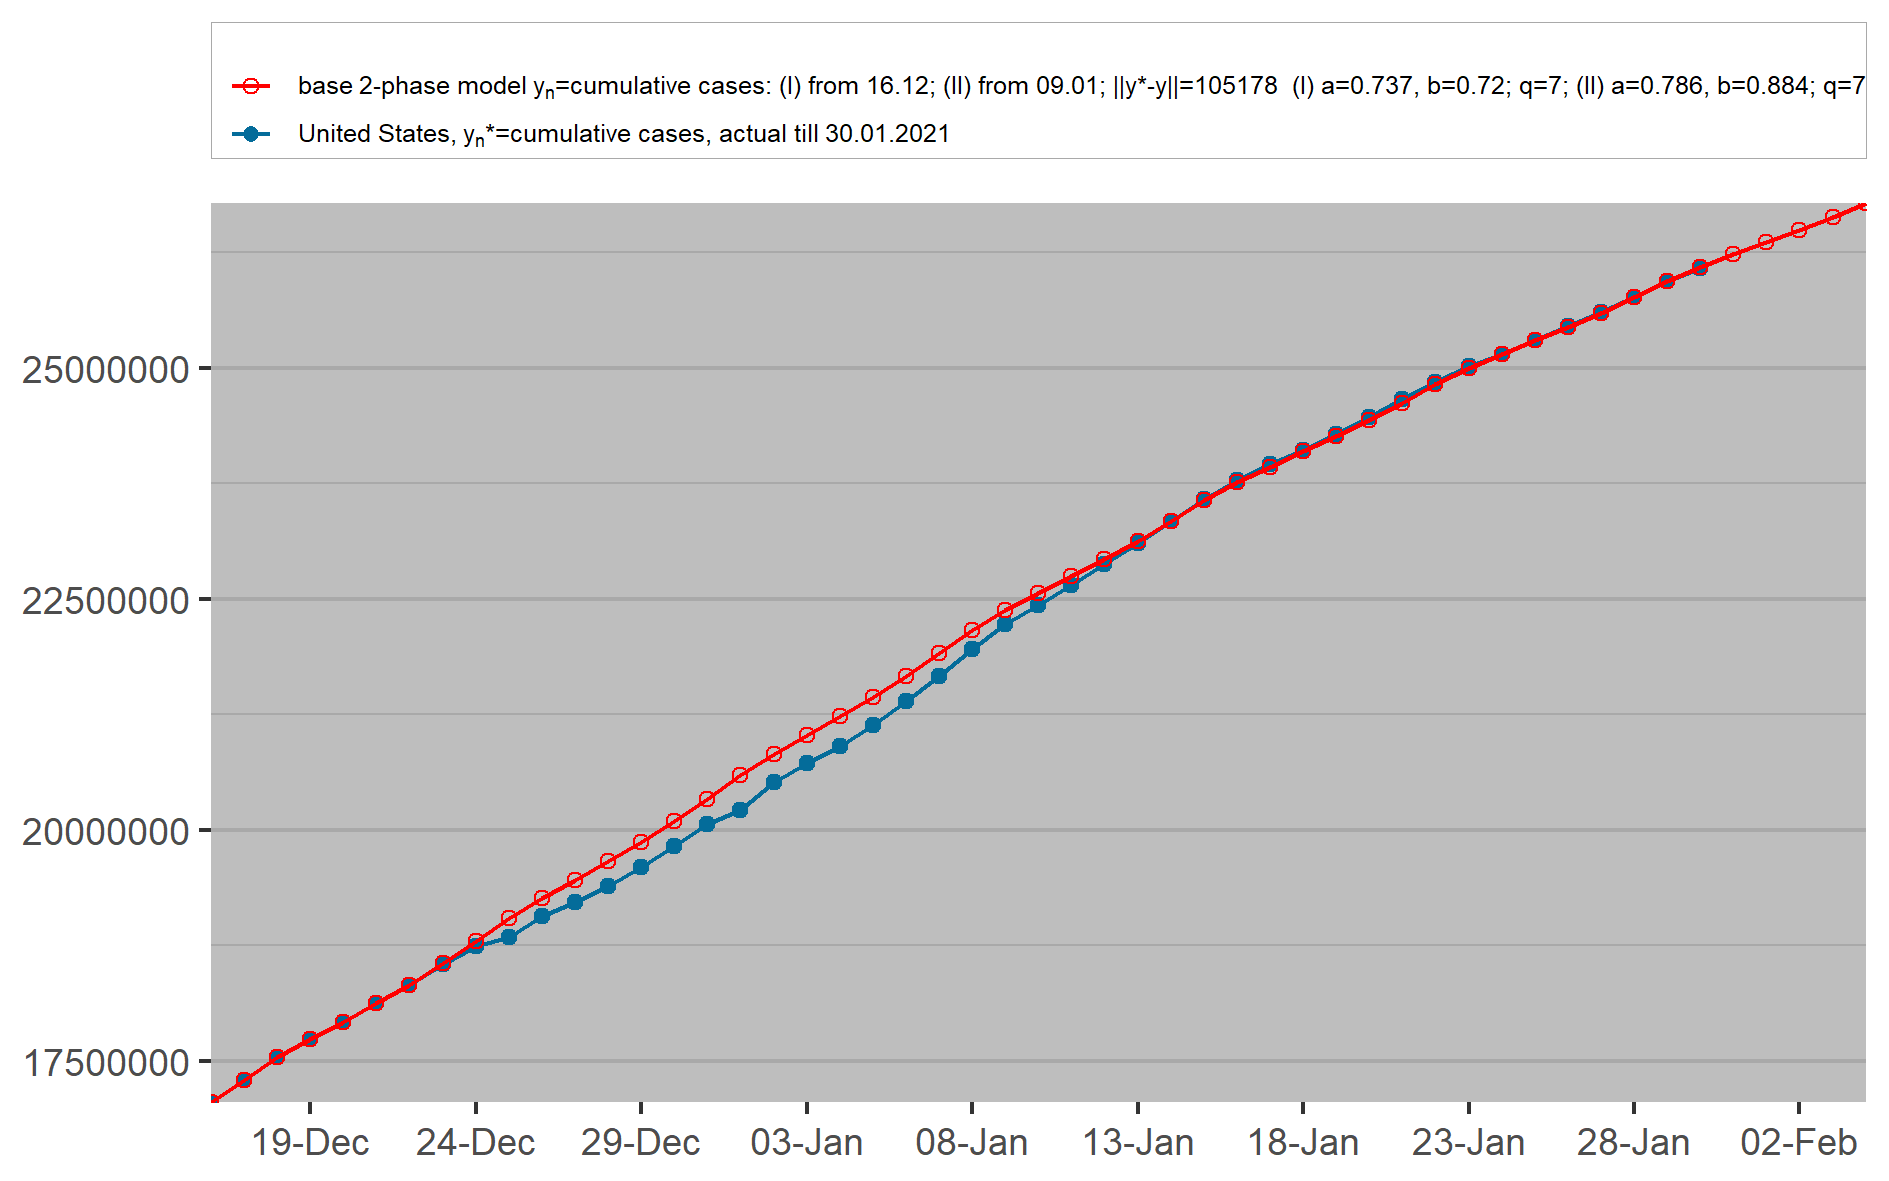
\includegraphics[width=\linewidth]{United States-ynmult.png} \label{fig:usa-ynmult}
\endminipage
\caption{Multi-phase model, United States}
\end{figure}

The periodic model often performs much better

\begin{figure}[H]
\minipage{0.48\textwidth}
  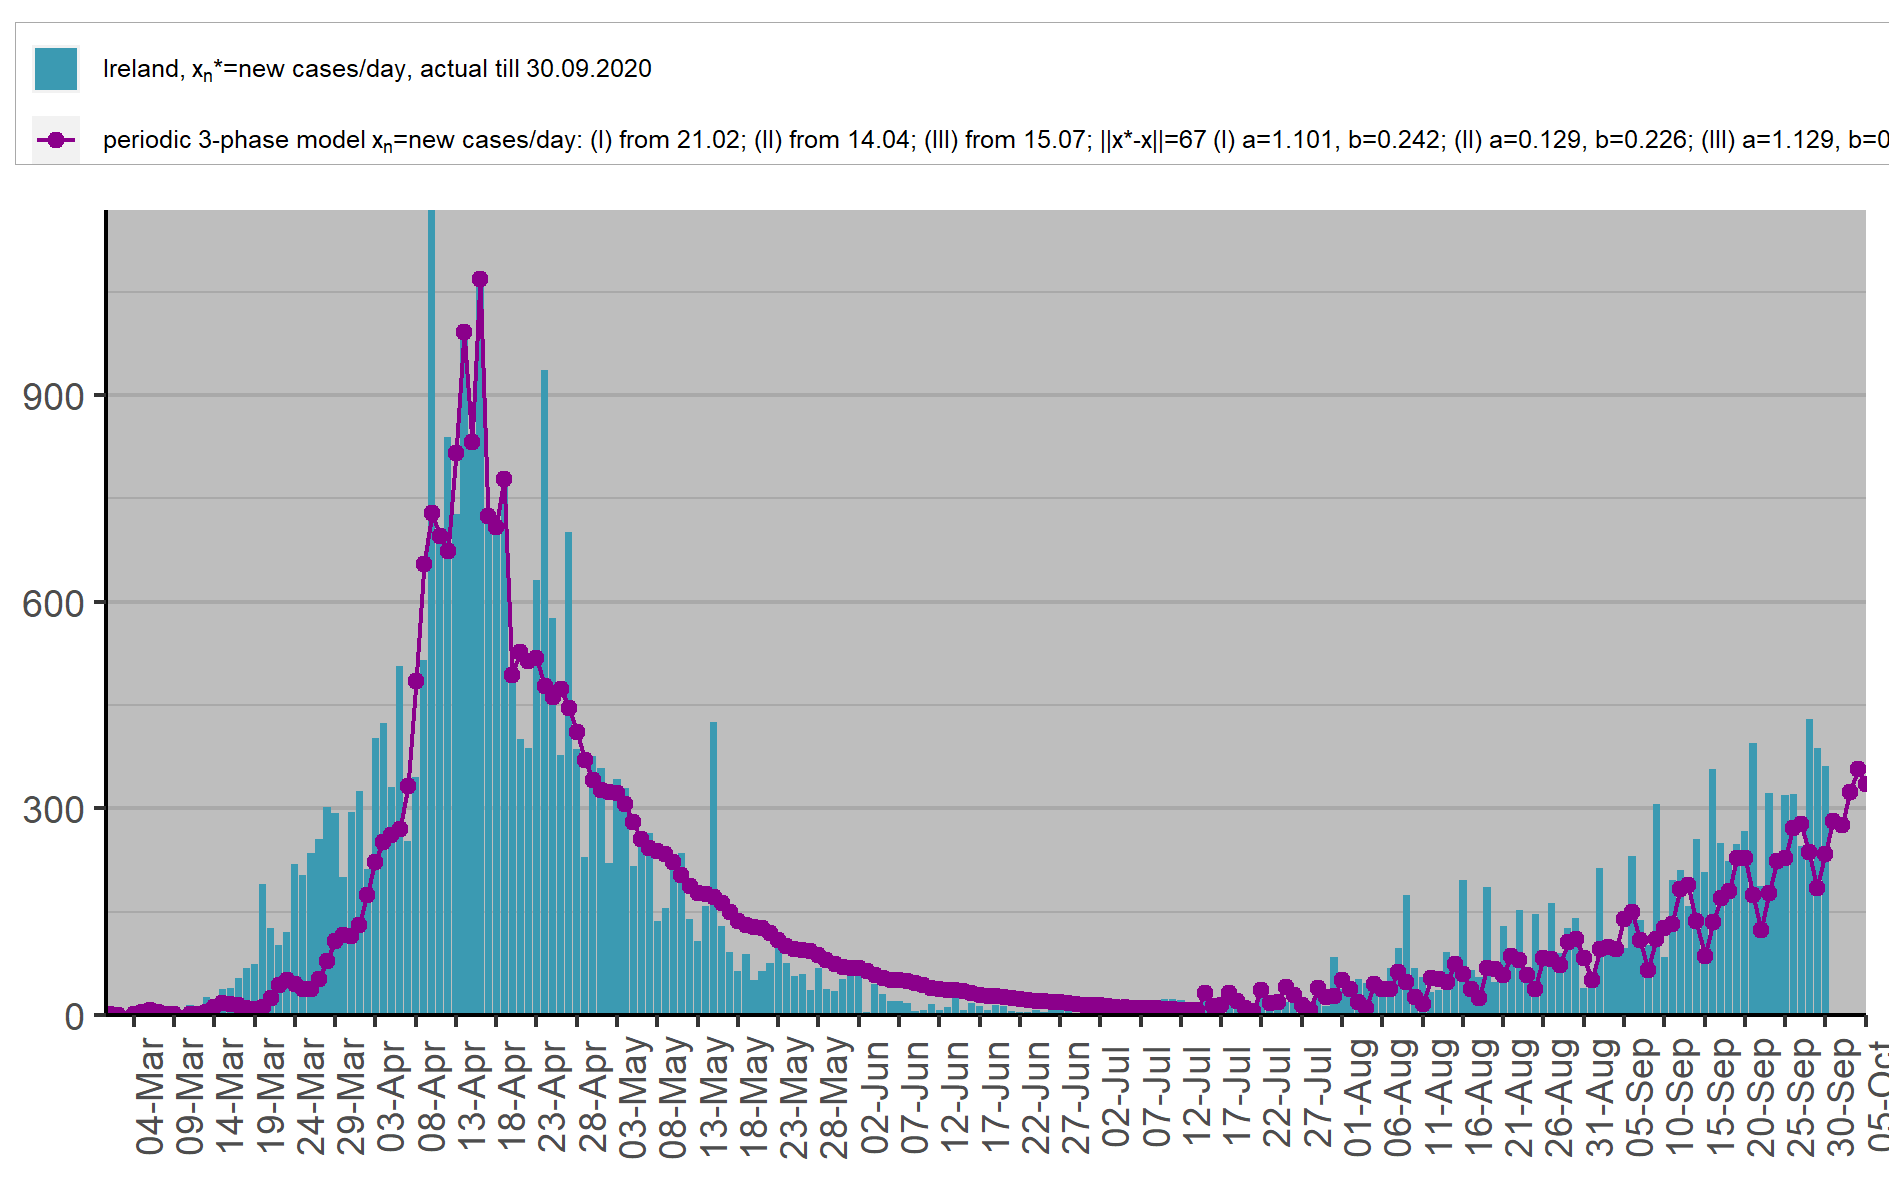
\includegraphics[width=\linewidth]{Ireland-perxnmult.png} \label{fig:ireland-perxnmult}
\endminipage\hfill
\minipage{0.48\textwidth}
  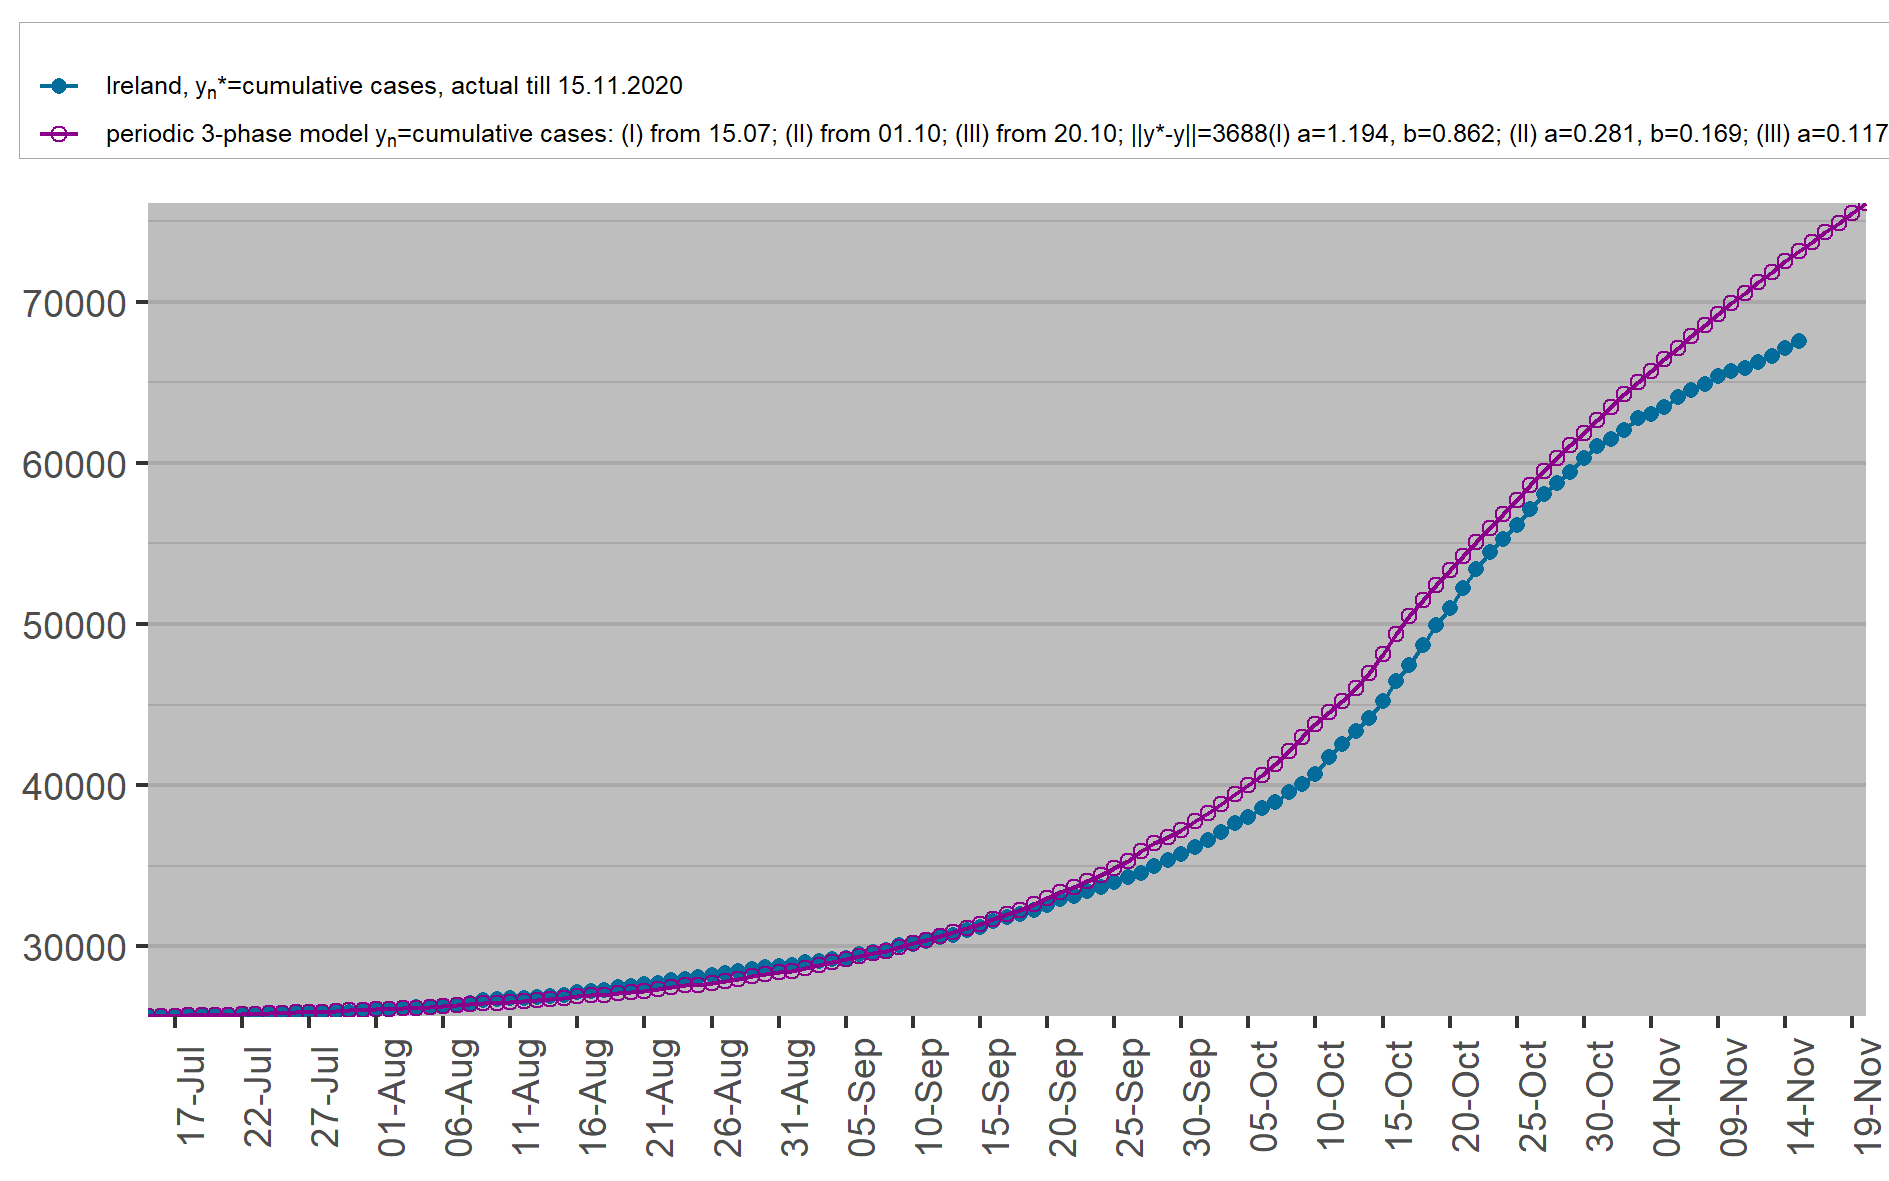
\includegraphics[width=\linewidth]{Ireland-perynmult.png} \label{fig:ireland-perynmult}
\endminipage
\caption{Multi-phase periodic model, Ireland}
\end{figure}

\begin{figure}[H]
\minipage{0.48\textwidth}
  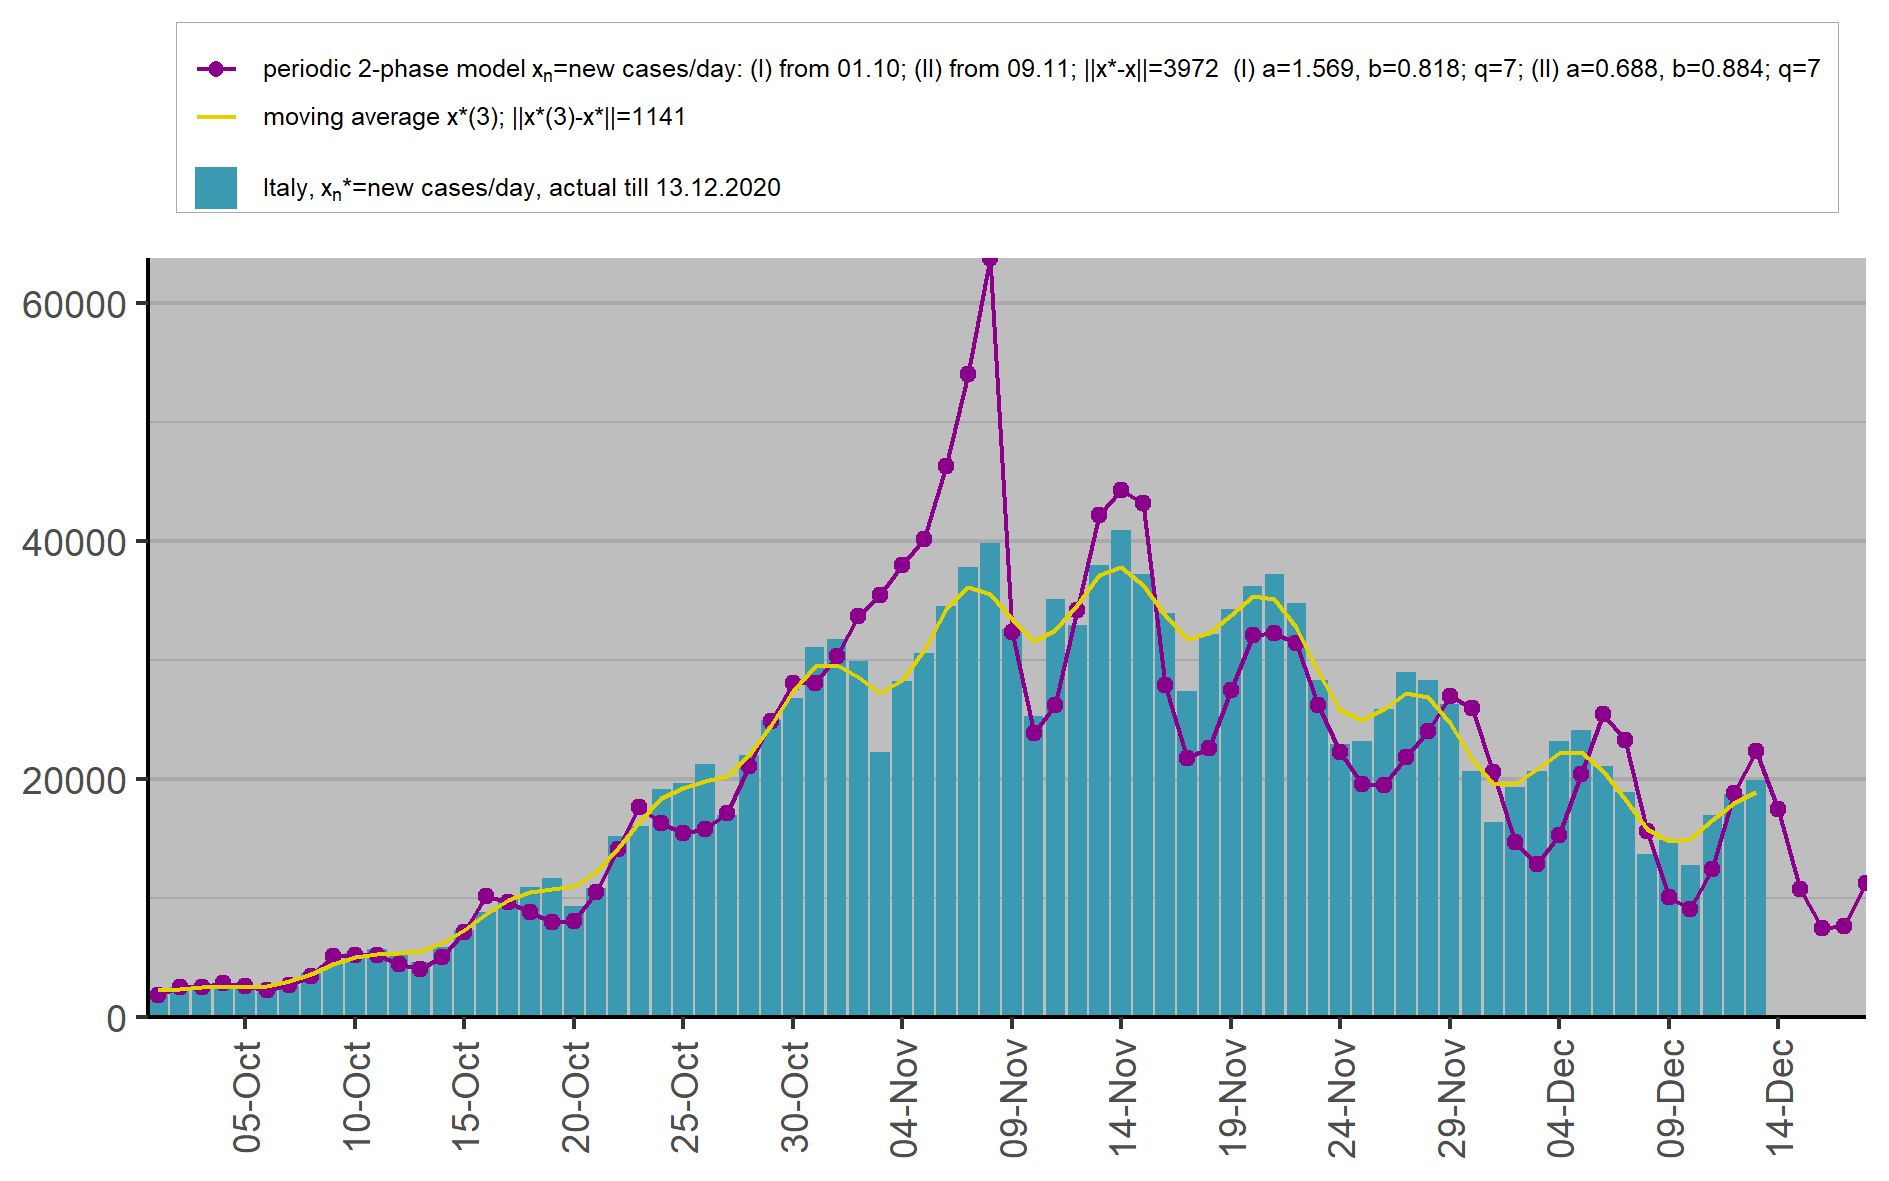
\includegraphics[width=\linewidth]{Italy-perxnmult.png} \label{fig:italy-perxnmult}
\endminipage\hfill
\minipage{0.48\textwidth}
  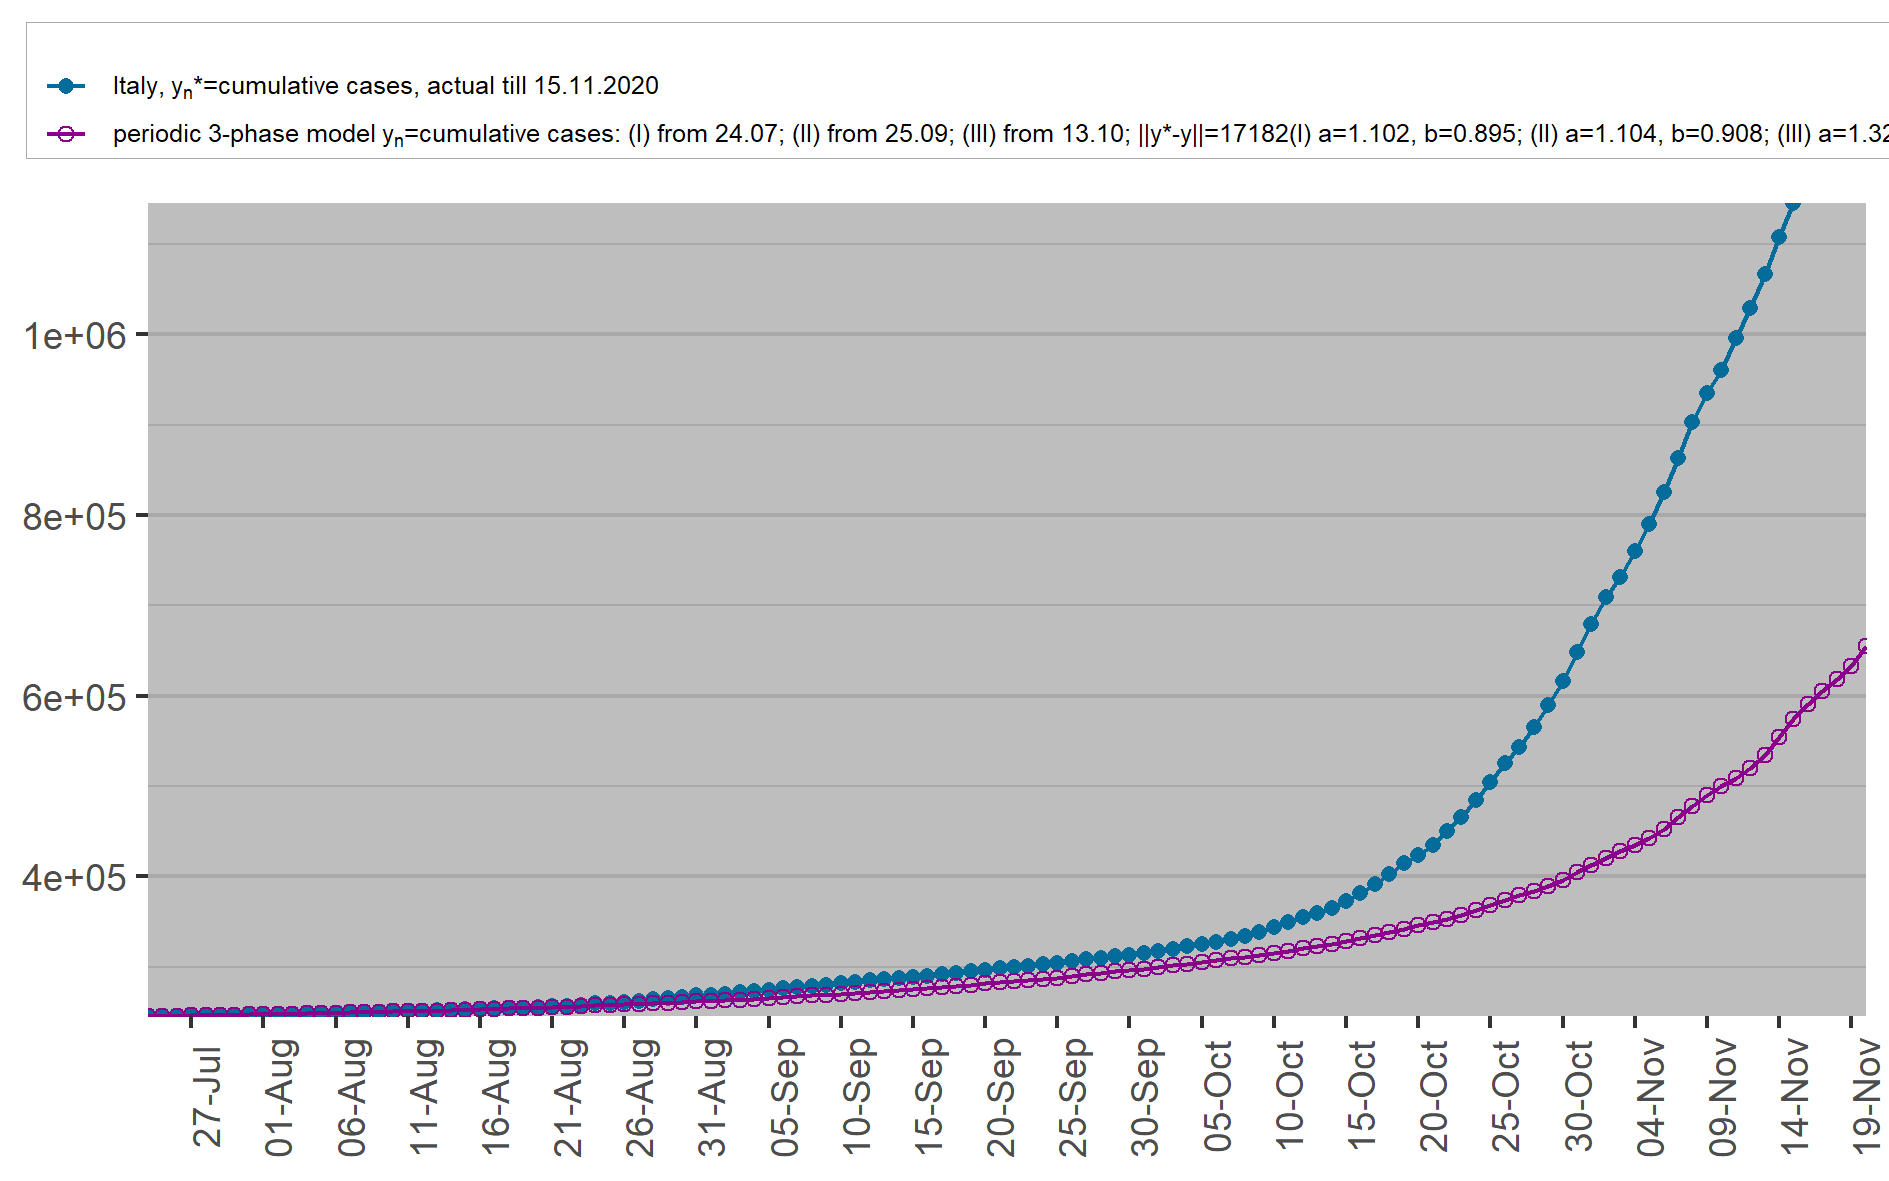
\includegraphics[width=\linewidth]{Italy-perynmult.png} \label{fig:italy-perynmult}
\endminipage
\caption{Multi-phase periodic model, Italy}
\end{figure}

\begin{figure}[H]
\minipage{0.48\textwidth}
  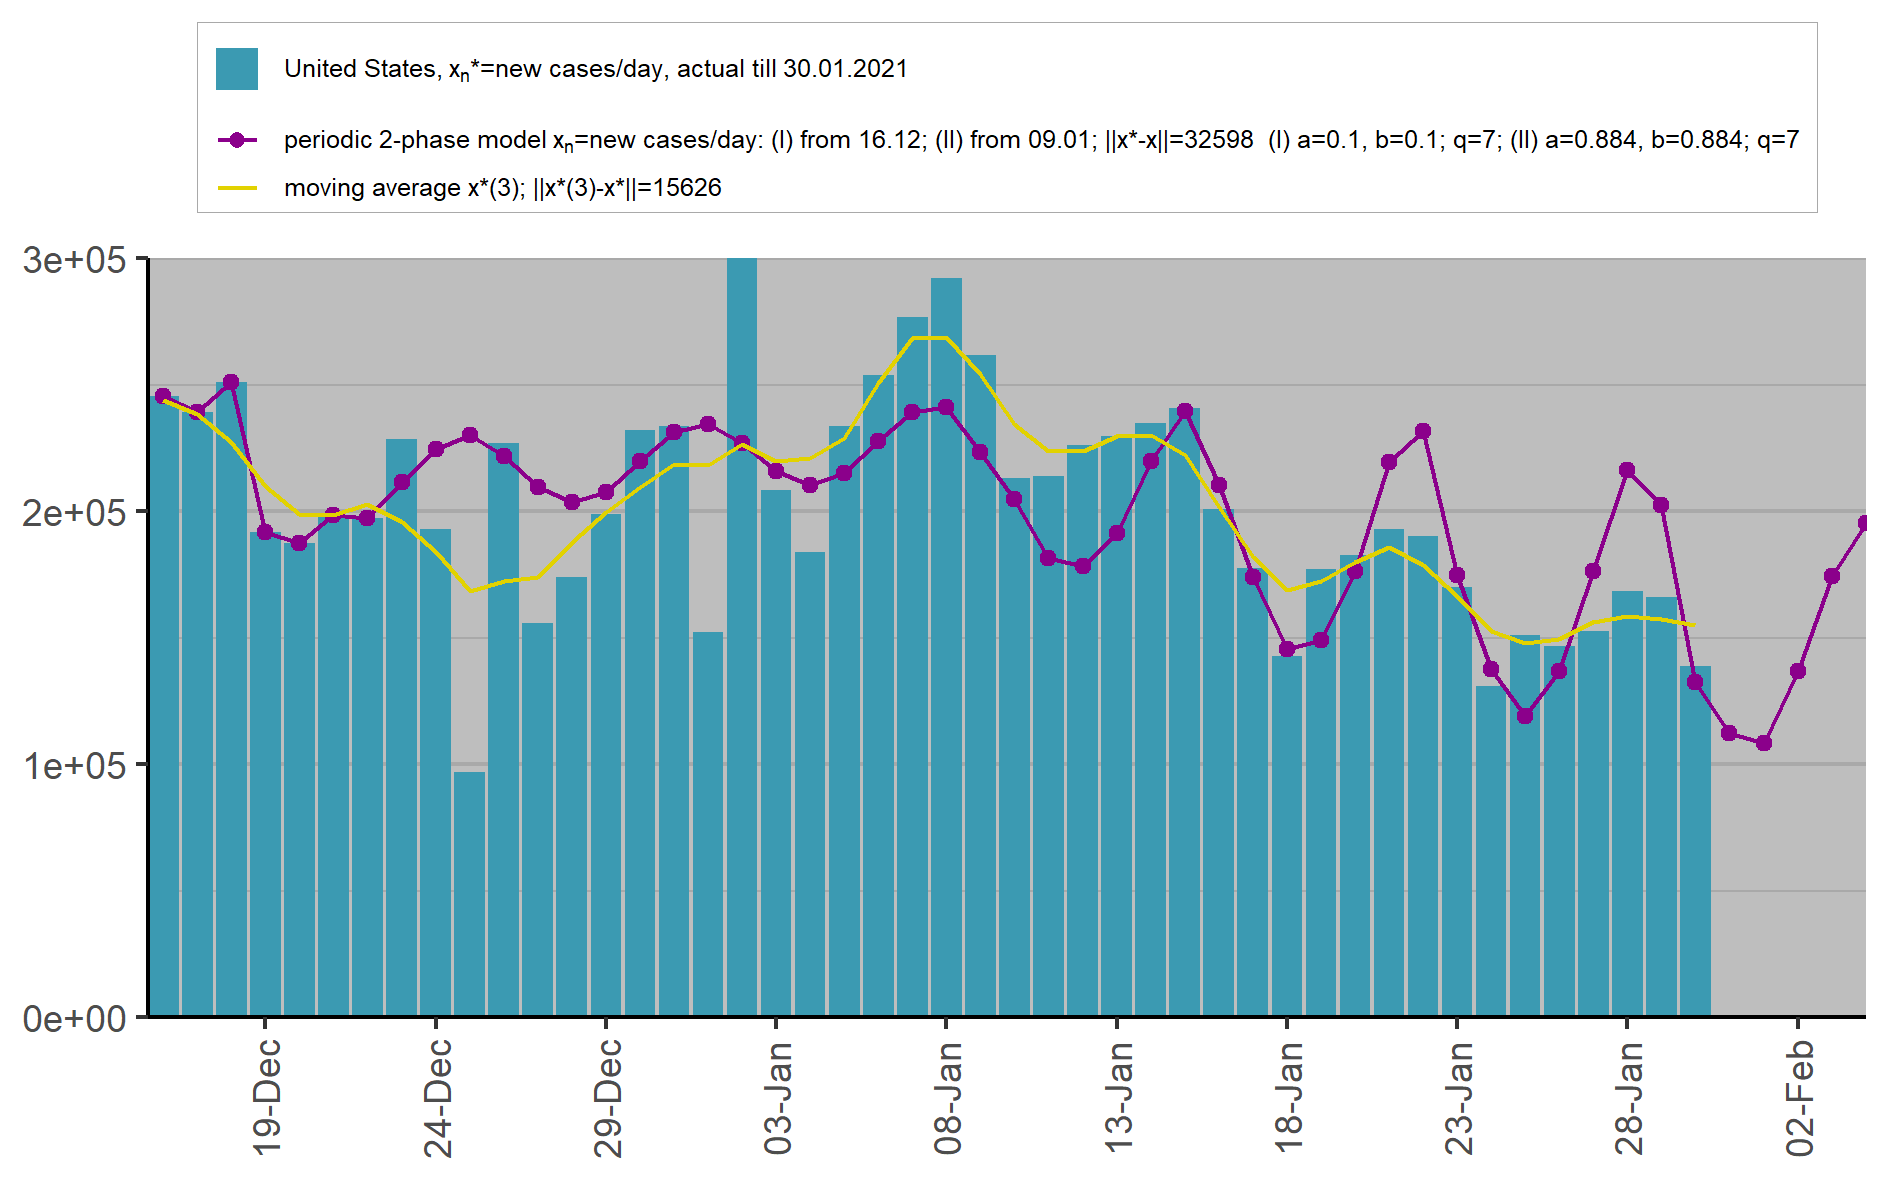
\includegraphics[width=\linewidth]{United States-perxnmult.png} \label{fig:usa-perxnmult}
\endminipage\hfill
\minipage{0.48\textwidth}
  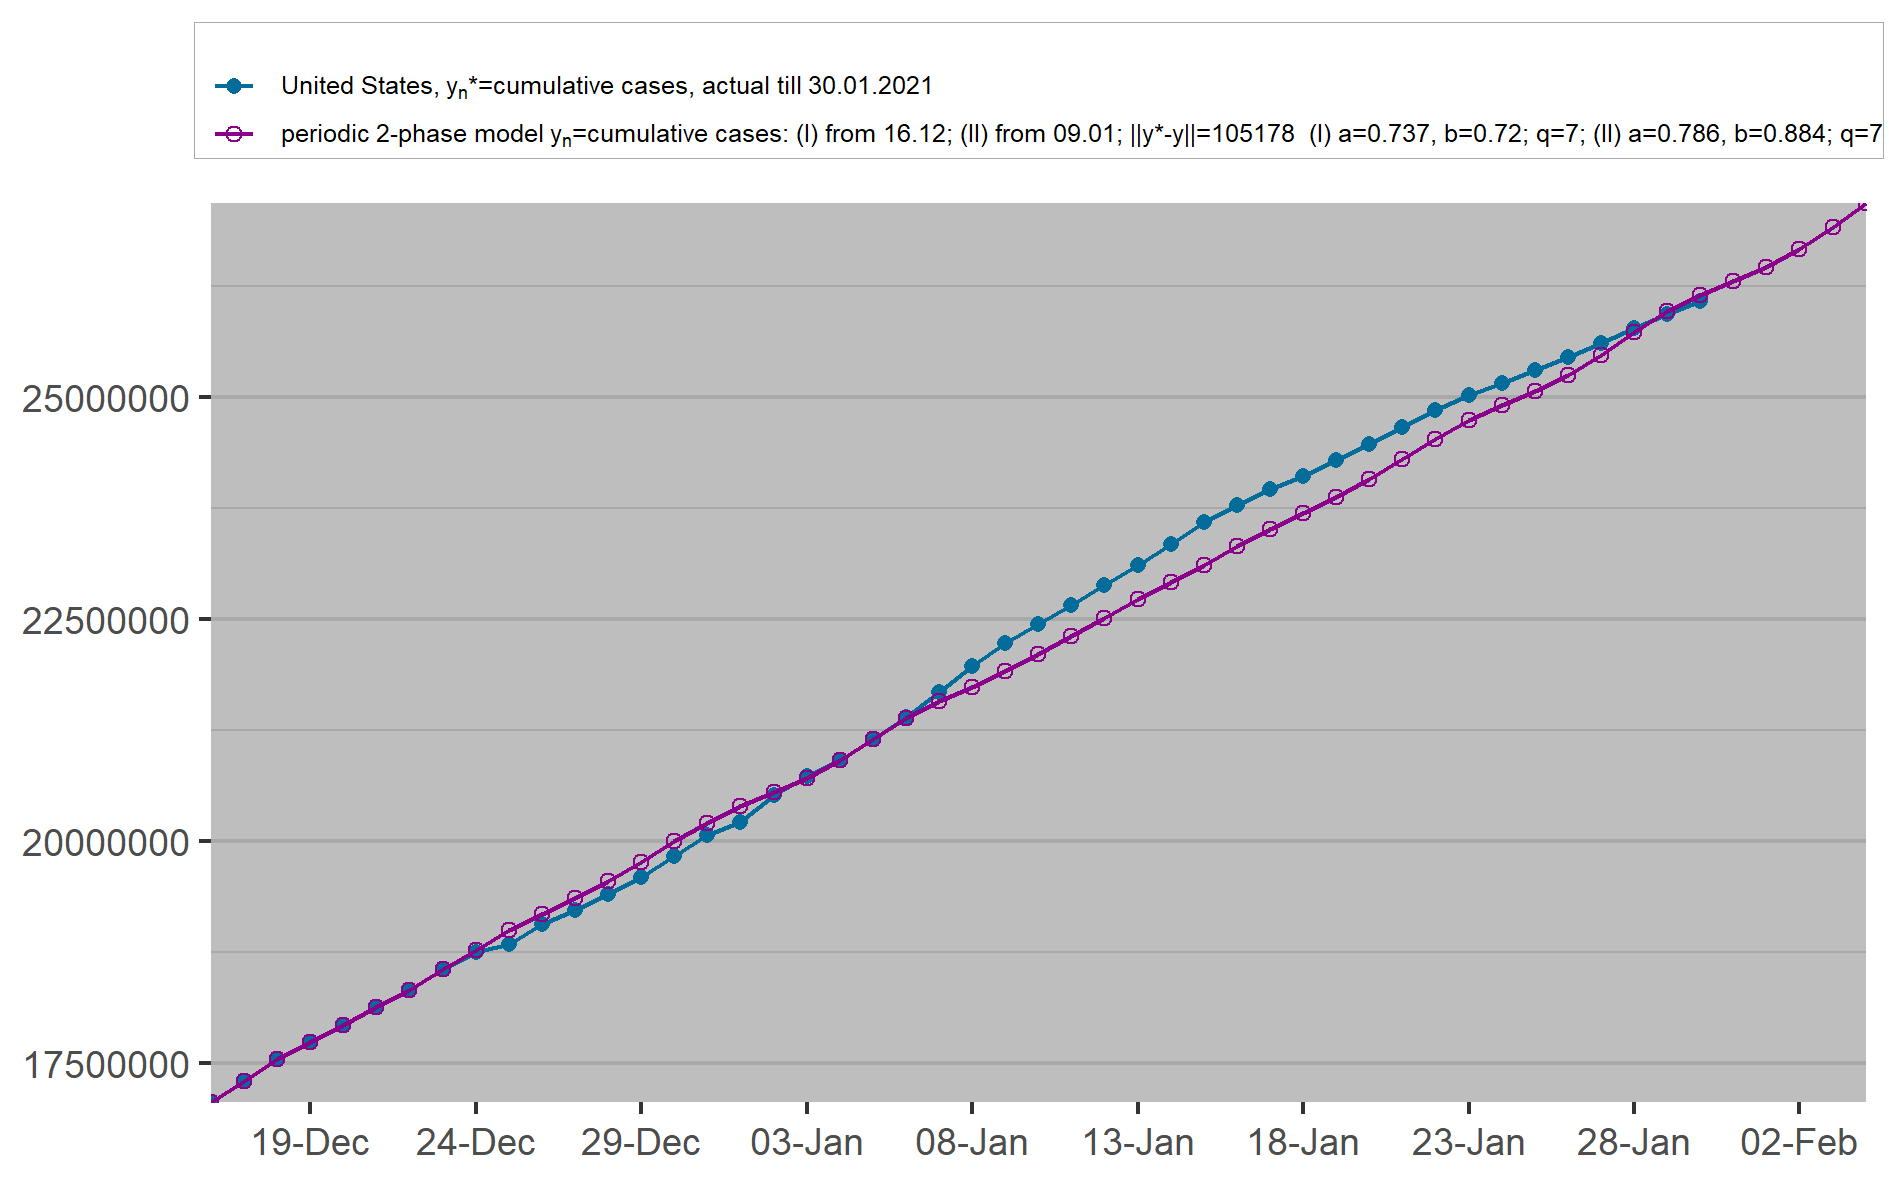
\includegraphics[width=\linewidth]{United States-perynmult.png} \label{fig:usa-perynmult}
\endminipage
\caption{Multi-phase periodic model, United States}
\end{figure}
